%%
% ?????????
%% This is file `sample-acmsmall.tex',
%% generated with the docstrip utility.
%%
%% The original source files were:
%%
%% samples.dtx  (with options: `acmsmall')
%%
%% IMPORTANT NOTICE:
%%
%% For the copyright see the source file.
%%
%% Any modified versions of this file must be renamed
%% with new filenames distinct from sample-acmsmall.tex.
%%
%% For distribution of the original source see the terms
%% for copying and modification in the file samples.dtx.
%%
%% This generated file may be distributed as long as the
%% original source files, as listed above, are part of the
%% same distribution. (The sources need not necessarily be
%% in the same archive or directory.)
%%
%% The first command in your LaTeX source must be the \documentclass command.
\documentclass[acmsmall]{acmart}
\usepackage{subfigure}

% \Cref
\usepackage{hyperref}
\usepackage{cleveref}

\usepackage{color}

%%
%% \BibTeX command to typeset BibTeX logo in the docs
\AtBeginDocument{%
  \providecommand\BibTeX{{%
    \normalfont B\kern-0.5em{\scshape i\kern-0.25em b}\kern-0.8em\TeX}}}

%% Rights management information.  This information is sent to you
%% when you complete the rights form.  These commands have SAMPLE
%% values in them; it is your responsibility as an author to replace
%% the commands and values with those provided to you when you
%% complete the rights form.
\setcopyright{acmcopyright}
\copyrightyear{2018}
\acmYear{2018}
\acmDOI{10.1145/1122445.1122456}


%%
%% These commands are for a JOURNAL article.
\acmJournal{JACM}
\acmVolume{37}
\acmNumber{4}
\acmArticle{111}
\acmMonth{8}

%%
%% Submission ID.
%% Use this when submitting an article to a sponsored event. You'll
%% receive a unique submission ID from the organizers
%% of the event, and this ID should be used as the parameter to this command.
%%\acmSubmissionID{123-A56-BU3}

%%
%% The majority of ACM publications use numbered citations and
%% references.  The command \citestyle{authoryear} switches to the
%% "author year" style.
%%
%% If you are preparing content for an event
%% sponsored by ACM SIGGRAPH, you must use the "author year" style of
%% citations and references.
%% Uncommenting
%% the next command will enable that style.
%%\citestyle{acmauthoryear}

%%
%% end of the preamble, start of the body of the document source.
\begin{document}

%%
%% The "title" command has an optional parameter,
%% allowing the author to define a "short title" to be used in page headers.
\title{JDAN: Joint Detection and Association Network for Real-Time Online Multi-Object Tracking}

%%
%% The "author" command and its associated commands are used to define
%% the authors and their affiliations.
%% Of note is the shared affiliation of the first two authors, and the
%% "authornote" and "authornotemark" commands
%% used to denote shared contribution to the research.
\author{Haidong Wang}
\email{haidong@hnu.edu.cn}
\affiliation{%
  \institution{Hunan University}
  \country{China}
}
\author{Xuan He}
\email{419432961@qq.com}
\affiliation{%
	\institution{Hunan University}
	\country{China}
}
\author{Zhiyong Li*}
\email{zhiyong.li@hnu.edu.cn}
\affiliation{%
  \institution{Hunan University}
  \country{China}
}
\author{Jin Yuan*}
\email{yuanjin@hnu.edu.cn}
\affiliation{%
  \institution{Hunan University}
  \country{China}
}
\author{Shutao Li}
\email{shutao_li@hnu.edu.cn}
\affiliation{%
  \institution{Hunan University}
  \country{China}
}

%%
%% By default, the full list of authors will be used in the page
%% headers. Often, this list is too long, and will overlap
%% other information printed in the page headers. This command allows
%% the author to define a more concise list
%% of authors' names for this purpose.
\renewcommand{\shortauthors}{H. Wang and Z. Li, et al.}

%%
%% The abstract is a short summary of the work to be presented in the
%% article.
\begin{abstract}
In the last few years, enormous strides have been made for object detection and data association that are vital subtasks for one-stage online multi-object tracking (MOT). 
However, the two separated submodules involved in the whole MOT pipeline are processed or optimized separately, resulting in a complex method design and requiring manual settings. 
In addition, few works integrate the two subtasks into a single end-to-end network to optimize the overall task. 
In this study, we propose an end-to-end MOT network named joint detection and association network (JDAN) that is trained and inferred in a single network. 
All layers in JDAN are differentiable, and can be optimized jointly to detect targets and output an {association} matrix for robust multi-object tracking. 
What's more, we generate suitable pseudo labels to address the data inconsistency between object detection and association. 
The detection and association submodules could be optimized by the composite loss function that is derived from the detection results and the generated pseudo association labels, respectively. 
The proposed approach is evaluated on two MOT challenge datasets, 
and achieves promising performance compared with classic and latest methods. 
\end{abstract}

%%
%% The code below is generated by the tool at http://dl.acm.org/ccs.cfm.
%% Please copy and paste the code instead of the example below.
%%
\begin{CCSXML}
	<ccs2012>
	<concept>
	<concept_id>10010147.10010257.10010258.10010259.10010263</concept_id>
	<concept_desc>Computing methodologies~Supervised learning by classification</concept_desc>
	<concept_significance>300</concept_significance>
	</concept>
	<concept>
	<concept_id>10010520.10010570.10010574</concept_id>
	<concept_desc>Computer systems organization~Real-time system architecture</concept_desc>
	<concept_significance>100</concept_significance>
	</concept>
	<concept>
	<concept_id>10010147.10010178.10010224.10010245.10010250</concept_id>
	<concept_desc>Computing methodologies~Object detection</concept_desc>
	<concept_significance>300</concept_significance>
	</concept>
	<concept>
	<concept_id>10010147.10010178.10010224.10010245.10010253</concept_id>
	<concept_desc>Computing methodologies~Tracking</concept_desc>
	<concept_significance>500</concept_significance>
	</concept>
	</ccs2012>
\end{CCSXML}


\ccsdesc[500]{Computing methodologies~Tracking}
\ccsdesc[300]{Computing methodologies~Object detection}
\ccsdesc[300]{Computing methodologies~Supervised learning by classification}
\ccsdesc[100]{Computer systems organization~Real-time system architecture}


%%
%% Keywords. The author(s) should pick words that accurately describe
%% the work being presented. Separate the keywords with commas.
\keywords{online multi-object tracking, end-to-end model, object detection and data association. }


%%
%% This command processes the author and affiliation and title
%% information and builds the first part of the formatted document.
\maketitle

\section{Introduction}
Online Multi-Object Tracking (MOT){, which aims to detect and track multiple targets in a sequence of video frames,} has attracted extensive attention in computer vision~\cite{an2021multitarget,RN1215,mahmoudi2019multi} {recently}. 
In practice, many applications benefit from the {success} of MOT tasks, such as intelligent driving~\cite{auto_driving}, video surveillance~\cite{deep_sort}, human activity recognition~\cite{mot16}{, and so on}. 
Currently, {there are} two kinds of mainstream MOT approaches, namely two-stage methods and one-stage methods. 
%\begin{figure}
%	\centering
%	\includegraphics[width=2.5in]{imgs/end-to-end.pdf}
%	\caption{
%		{End-to-end MOT model with object detection and data association.} 
%		The inputs of JDAN are the historical frame and current frame without detection results. 
%		Benefitting from the proposed JDAN, the detection and association results are generated directly. 
%	}
%	\label{fig:end-to-end}
%\end{figure}
% fairmot, 1, The state-of-the-arts
Two-stage methods~\cite{fang2018recurrent,nonlocal_association,poi} {usually} contain two independent stages{: detection and association}. 
The detection stage {adopts an offline training pattern, and aims to localize} the to-be-tracked targets in the current video frame. 
{Then,} the association stage extracts re-identification representations for the targets,
and matches them with the previous tracks. 
{Benefitting from the advances in detection~\cite{faster,point,redmon2018yolov3}, re-identification~\cite{k_reciprocal,expanded_re} and data association~\cite{nonlocal_association}, two-stage approaches have significantly improved the tracking accuracy for MOT task.}
Nevertheless, {as depicted in Fig.~\ref{fig:consistency}~(a), this paradigm first requires an offline detection, and then repeats feature extraction to generate trajectories.
Therefore, it is difficult to implement a real-time tracking.
}
%due to the complex process as well as the repetitive feature extraction, the two-stage pipeline} is difficult to achieve real-time MOT tracking.
% limitation of the lack of sharing of the parameter in the two-stage model, it is difficult to achieve real-time MOT tracking. 

\begin{figure}[t]
	\centering
	\includegraphics[width=5.2in]{imgs/consistency.pdf}
	\caption{
		{An explanation of two-stage MOT, one-stage MOT and our \emph{end-to-end} MOT. 
		(a) Traditional two-stage MOT pipeline contains two separate stages and extract feature twice.
%		Thus, it is difficult to achieve real-time MOT tracking.
		(b) Existing one-stage MOT pipeline adopts an independent processing pattern for detection and association during the training process, 
		and could not achieve an \emph{end-to-end} training. 
%		with complex and hand-designed methods to associate objects.
%		But it is difficult to capture the association complexities in the real world. 
		(c) Our proposed \emph{end-to-end} MOT model integrates object detection and data association into a one-stage MOT tracker, 
		and uses a traditional association method~\cite{welch1995introduction} to generate pseudo association labels, which are utilized to keep data consistency between object representations and association labels in each training iteration.
		}
		%		There are many inconsistent bounding boxes, including the number and the position between the bounding box ground truth~\cite{dpm,faster,sdp} and the output of our \emph{detection submodule} in the MOT benchmark datasets. 
		%		While the training data provided in the MOT benchmark dataset lack the implementation of these detection models, it is necessary to implement a one-stage MOT, as depicted in Sec.~\ref{sec:two_stage} and \emph{end-to-end} MOT. 
	}
	\label{fig:consistency}
\end{figure}

% fairmot, 1, With the maturity
{Different from two-stage approaches, one-stage methods~\cite{jde,voigtlaender2019mots} try to integrate both \emph{online} detection and association into one framework, } 
{and thus could} share model parameters for target {representations (see Fig.~\ref{fig:consistency} (b)) to} decrease the tracking cost~\cite{jde,memory_improved}. 
%However, compared with the two-stage approaches, several drawbacks prevent the implementation of {an} \emph{end-to-end} MOT model. 
{
However, common one-stage methods adopt an independent processing pattern for detection and association,
including training an effective detection model and then employing complex association tricks for generating trajectories. 
The association results greatly depend on the detection accuracy.
In other words, detection and association are independent of each other during the training process, 
and could not achieve an \emph{end-to-end} training.
As a result, object detection errors will be propagated to the association stage, thereby reducing the accuracy of MOT. 
}


{
Motivated by the above analysis, this paper proposes an \emph{end-to-end} training framework named "Joint Detection and Association Network" ("JDAN" for short) to alleviate this problem. 
Our framework mainly consists of three parts: \emph{detection submodule}, \emph{joint submodule}, and \emph{association submodule}. 
Concretely, we first use a pre-trained two-stream detection network to extract initial object candidates and their representations. 
Then, the \emph{joint submodule} is employed to merge all possible representation concatenations between two frames to generate a \emph{confusion tensor}. 
Finally, the \emph{association submodule} converts the tensor to an \emph{association matrix}, which indicates the matching relation among multiple targets from the two frames. 
To jointly train the previous submodules, one challenge lies in the inconsistent object problem,
where the \emph{detection submodule} may generate inconsistent objects in quality, location and size as compared to the tracking ground truth for MOT task. 
To bridge this gap, our approach abandons the existing tracking ground truth,
and leverages the traditional association method~\cite{welch1995introduction} to produce pseudo labels for detection results (see Fig.~\ref{fig:consistency} (c)), 
which are then fed to the \emph{association submodule} to generate tracking results. 
Consequently, our model could jointly train all the submodules in an \emph{end-to-end} way to generate a robust one-stage model. 
Moreover, as pseudo labels are only used in the training stage instead of testing, they have no effect in prediction speed during the inference stage.
}
%to obtain the required \emph{association matrix}.
%However, as the training process continues, different \emph{detection submodule} parameters have different detection results which are inconsistent with the MOT benchmark datasets in number, location and size. 
%Meanwhile, the inferred object representations of the \emph{detection submodule} do not have corresponding association labels.
%To solve the problem of data inconsistency between object representations and association labels, we utilize the traditional association method \cite{fairmot} to produce pseudo labels, as depicted in Fig.\ref{fig:consistency} (c).
%And these pseudo-labels are only used in the training process, and have no effect on the inference speed of the model. 


%These factors make it impossible to obtain a single \emph{end-to-end} MOT model. 
% the precision of one-stage MOT algorithms is not satisfactory. 
% fairmot, 1, Instread, Three factors
% fairmot, 1, (1), However, the anchors
%{First, there are modality differences between object detection and data association~\cite{gu2019temporal}}. 
%The former only involves the processing of spatial information, while the latter concerns data association over time series. 
%These differences make the design of the \emph{end-to-end} MOT model more difficult. 
% Thus, when we design the detection submodule, multi-layer representation~\cite{point} is necessary. 
% anchor box is improper to object association, because many anchor boxes may correspond to the same target. 
% Another reason is that the repeated downsample representation is quite rough for object association~\cite{point}. 
% fairmot, 1, (2) This is particularly
%{Second, the existing bounding box labels in two-stage MOT dataset have no consistent detection results compared with our own detection module.} 
%{Second, as the training process continues, different \emph{detection submodule} parameter have different detection results for a specified frame.
%}
%{So we can not use existing detection results and association labels in MOT benchmark datasets.}
%the feature inconsistency of bounding box between the output of the detection model and the input of the association model prevents the training process in the whole \emph{end-to-end} MOT model, as depicted in Fig.\ref{fig:consistency}(c). 
%{Thus, data consistency between the object representations and association labels must be achieved when training.} 
% Then, object representations require to be able to take advantage of low and high resolution representations to adapt big and small targets simultaneously. 
% fairmot, 1, (3), Learning low-dimensional
%{In addition, as the training process continues, the inferred object representation of the \emph{detection submodule} do not have corresponding associated labels.}
%These factors make it impossible to obtain a single \emph{end-to-end} MOT model. 
% In addition, object representations with a lower dimension are more suitable for MOT, because the training set of MOT is too small to cause the under-fitting of network. 
% fairmot, 1, We present, a 


%{Based on the above analysis, we seek to solve these knotty problems 
%and propose an \emph{end-to-end} MOT method that is jointly responsible for object detection and data association.} 
%% Based on previous works, FairMOT~\cite{fairmot} proposes a brief method that considers these reasons together when extract the object representation, 
%% fairmot 1, We present a 
%% However, facing the challenges of long inter-frame object occlusions and complex MOT scenarios, it is far from enough to focus on model connection alone. 
%% Note that we do not
%{To solve the problem of modality differences between object and data association, we proposed a two-stream detection network and \emph{joint submodule} for a pair of video frame separated by $n$ time stamps, as depicted in Fig.~\ref{fig:pipeline}.}
%%{The proposed MOT pipeline is depicted in Fig.~\ref{fig:consistency}(c) and Fig.~\ref{fig:pipeline}.} 
%%In addition, we exploit the existing object detection and data association method to design submodules that meet our requirements. 
%%{As depicted in Fig.\ref{fig:consistency}, to utilize our \emph{detection submodule}, there are many inconsistent boxes between the existing labels in MOT benchmark datasets and the results of our proposed \emph{detection submodule} for input video frames $F$.} 
%{In addition, to solve the problem of data inconsistency between object representations and association labels, we first train our \emph{detection submodule} on the detection datasets~\cite{zhang2017citypersons,ess2008mobile} in training stage 1, 
%and then use the trained \emph{detection submodule} to generate corresponding bounding boxes, 
%and utilize the traditional association method {~\cite{fairmot}} to produce pseudo association labels. 
%Therefore, these pseudo labels can be utilized to train our \emph{association submodule} in training stage 2 by the fixed parameter of \emph{detection submodule}, as depicted in Fig.\ref{fig:consistency}(c).
%}
%Finally, the \emph{online} MOT is performed by associating the current frame with several separate historical frames apart using the output of \emph{association submodule}. 
%{Thus, these strategies can realize the data consistency to complete our training and \emph{end-to-end} real-time detection tracking.} 

{
Different from previous one-stage methods, our approach could jointly train both \emph{detection} and \emph{association submodules} in an \emph{end-to-end} fashion,
which alleviates the error propagation problem. 
% fairmot, 1, We evalute our approach
We evaluate the proposed method on MOT15~\cite{taix2015motchallenge} and MOT17~\cite{mot16} datasets, 
and find the proposed method outperforms multiple \emph{online} trackers.
}
%In addition to the high precision, the \emph{end-to-end} method is simple and suitable for use in real time. 
We believe that this study will be a good inspiration for one-stage \emph{online} MOT. 



To sum up, our primary contributions are listed below:
{
\begin{enumerate} 
	\item {We propose an \emph{end-to-end} architecture to jointly process both object detection and association to alleviate the error propagation problem. To the best of our knowledge, our work is the first attempt to implement an \emph{end-to-end} training for MOT task.}
	\item {Our approach employs pseudo labels to solve the object inconsistent problem, and we propose a \emph{joint submodule} followed by association prediction to produce precise tracking results based on these pseudo samples.}
	\item {We conduct abundant experiments on MOT benchmark datasets with ablation study. It is demonstrated that our approach could implement a real-time \emph{online} tracking as well as achieve competitive tracking performance as compared to several popular models.}
\end{enumerate}
}
%	\item {An \emph{end-to-end} architecture is designed to process the object detection and \emph{online} MOT task jointly and 
%	alleviates the problem of detection error propagation.} 
%	\item {A \emph{joint submodule} and a suitable generaration method of pseudo labels are proposed to solve the data inconsistent problem between the object representation of the \emph{detection submodule} and the association label of the \emph{association submodule}.} 
%	\item We design a two stage training method to train the \emph{detection submodule} and the \emph{association submodule}, and perform the online MOT process in an \emph{end-to-end} mode completely. 
%	\item Abundant experiments are performed on MOT benchmark datasets with ablation study, 
%	{and the proposed algorithm combining the advantages of the two-stage method and the one-stage method obtains competitive tracking accuracy against many \emph{online} MOT approaches.} 



\section{related work} \label{related work}
% fairmot, 2, In this section,
We summarize several recent research progress on \emph{online} MOT by grouping them into two-stage and one-stage approaches, 
and analyze the advantages and disadvantages of these approaches. 

\subsection{Two-Stage MOT Approaches}
Traditional tracking algorithms~\cite{deep_sort,mahmoudi2019multi,zhou2018online,poi} usually consider object detection and data association as two independent stages: 
{First, they utilize the object detection technology to find all targets for each video frame in the form of bounding boxes~\cite{he2017mask,redmon2018yolov3,luo2020strong}}; 
%they clip the video frame according to the detection results. 
Second, they conventionally follow a typical paradigm that computes a similarity loss according to the spatial relationship and appearance representation of detection results, 
and then perform state estimation~\cite{welch1995introduction,multi_pattern,weight_sparse,local_sparse,RN1215} and data association~\cite{kuhn1955hungarian,zhou2018online} to solve the association problem across video frames to generate a series of trajectories. 
To improve the performance, advanced studies~\cite{mahmoudi2019multi} utilize sophisticated associative methods such as recurrent neural network~\cite{fang2018recurrent} and graph matching~\cite{zhou2018online}. 
%
The merit of these two-stage approaches is that they can utilize the most appropriate method for each stage respectively to maximize the performance. 
What's more, they clip video frames based on detected bounding boxes and resize them to the same scale before learning object representations, 
which contributes to dealing with the scale difference problem of tracked targets. 
Generally, two-stage methods~\cite{poi} could achieve the optimum tracking performance on MOT benchmarks, 
but are quite time-consuming since both detection and representation extraction require abundant computing resource. 
Hence, it is very difficult to obtain a real-time tracking.
% such tracking is necessary in many real scenes. 

% fairmot, 2.2, 
\subsection{One-Stage MOT Approaches}
With the development of object detection~\cite{xu2021exploring} and multi-task learning~\cite{ranjan2017hyperface,kokkinos2017ubernet}, a recent trend in MOT {tries} to combine both detection and data association into a single framework, 
with the aim of reducing the runtime by using shared parameters. 
For instance, {MOTS}~\cite{voigtlaender2019mots} appends a re-identification branch based on {mask R-CNN}~\cite{he2017mask} to predict bounding boxes{, and uses a fully connected layer to predict an association vector for each proposal based on additional image segmentations}. 
Moreover, JDE~\cite{jde} built on YOLOv3~\cite{redmon2018yolov3} could obtain a high tracking speed, 
{
but the used anchors are not suitable for extracting object features in MOT task, resulting in a decreased accuracy. 
}
% fairmot, 2.2, We find this
{FairMOT~\cite{fairmot} uses the anchor-free approach to alleviate the problem of anchor-based methods.
However, detection and association are independent of each other during the training process, 
and thus it may cause detection error propagation. 
}
%discovers that the object embedding representations based on anchor boxes are not aligned with the target centers, producing severe ambiguity and many ID switches (\emph{ID\_Sw}). 
% fairmot, 2.2, However, the tracking
%because the one-stage approaches can't make full use of the best detection and association methods, especially the association method,
Typically, the performance of one-stage approaches is usually worse than that of the two-stage ones. 
{Moreover, since the data inconsistency between the two subtasks is not resolved, 
the previous methods could not implement an \emph{end-to-end} \emph{online} MOT.}  

{
Different from the previous approaches~\cite{fairmot,jde}, 
%we employ pseudo-labels to solve the object inconsistent problem between the two subtasks, 
our approach implements an \emph{end-to-end} architecture to jointly train both detection and association, 
and thus alleviates the error propagation problem as well as achieves a fast tracking. 
}
% fairmot, 2.2, To address the 
%To address these issues further, we develop a true \emph{end-to-end} approach to combine detection with data association that implements an \emph{end-to-end} model and increases the tracking speed and precision on MOT datasets to a certain extent. 

\section{Our Algorithm}
{
In this section, we first describe the framework of our proposed JDAN.
Then, we introduce the details including our \emph{detection submodule}, \emph{joint submodule} and \emph{association submodule}, respectively.
Finally, we present the training and testing strategies to formulate our \emph{end-to-end online} MOT.
}

%\subsection{Notations}
%The following notation is used in the paper.
%\begin{itemize}
%	\item $A$ indicates \emph{association matrix} that specifies the association probabilities between all targets in the current frame $F_t$ and all targets in the historical frame $F_{t-n}$.
%	\item $B_{t-n, t}$ is a \emph{binary association matrix} between historical and current frames as real labels.
%	\item $D$ represents the output of the \emph{displacement head}.
%	\item $E$ represents the generated representation map of the \emph{representation head}.
%	\item $F$, $F_t$, and $F_{t-n}$ represent any frame, current frame and previous $n$ frame,  respectively.
%	\item $M_t$, $M_{t-n}$, $M_{t-n,t}$ and $M_a$ are the representation tensor in the current frame, the representation tensor in the previous $n$ frame, the \emph{confusion tensor} between the current frame and previous $n$ frame, and the \emph{association matrix}, respectively.
%	\item $N_m$ represents the maximum number of tracked objects in every video frame. 
%	\item $R_t$ and $R_{t-n}$ are the represention matrices in the currrent frame and previous $n$ frame, respectively. 
%	\item $S_D$, $S_A$ and $S_J$ represent the object \emph{detection submodule}, data \emph{association submodule} and detection-tracking \emph{joint submodule}, respectively.
%\end{itemize}

\subsection{Framework}

{
Fig.~\ref{fig:pipeline} demonstrates the framework of our proposed JDAN,
which mainly consists of three submodules: \emph{detection submodule}, \emph{joint submodule}, and \emph{association submodule}.
First, two input video frames are disposed of the two-stream \emph{detection submodule} with shared parameters to learn object representations. 
On this basis, all object representations are then copied along the vertical and horizontal directions, respectively, to form a \emph{confusion tensor} in \emph{joint submodule}. 
Finally, the generated tensor is converted into an \emph{association matrix} via an \emph{association predictor} in the \emph{association submodule}. 
As a result, the matching relationship between multiple targets from the two frames is predicted according to the \emph{association matrix}.
%In the end, the \emph{association matrix} is utilized to perform \emph{online} MOT by reviewing the historical video frames.
Different from previous approaches, our algorithm could solve the data inconsistent problem between detection and tracking tasks, and implement an \emph{end-to-end} training pattern to alleviate the error propagation problem. 
} 
%{Then, we introduce our \emph{joint submodule}, training strategy and solutions to data inconsistency}. 
%{Finally, we present the \emph{association submodule}, the design of loss function and \emph{online} tracking strategy to formulate the \emph{end-to-end} MOT.} 

% Learning a Neural Solver for, 3, Our methods

\begin{figure*}
	\centering
	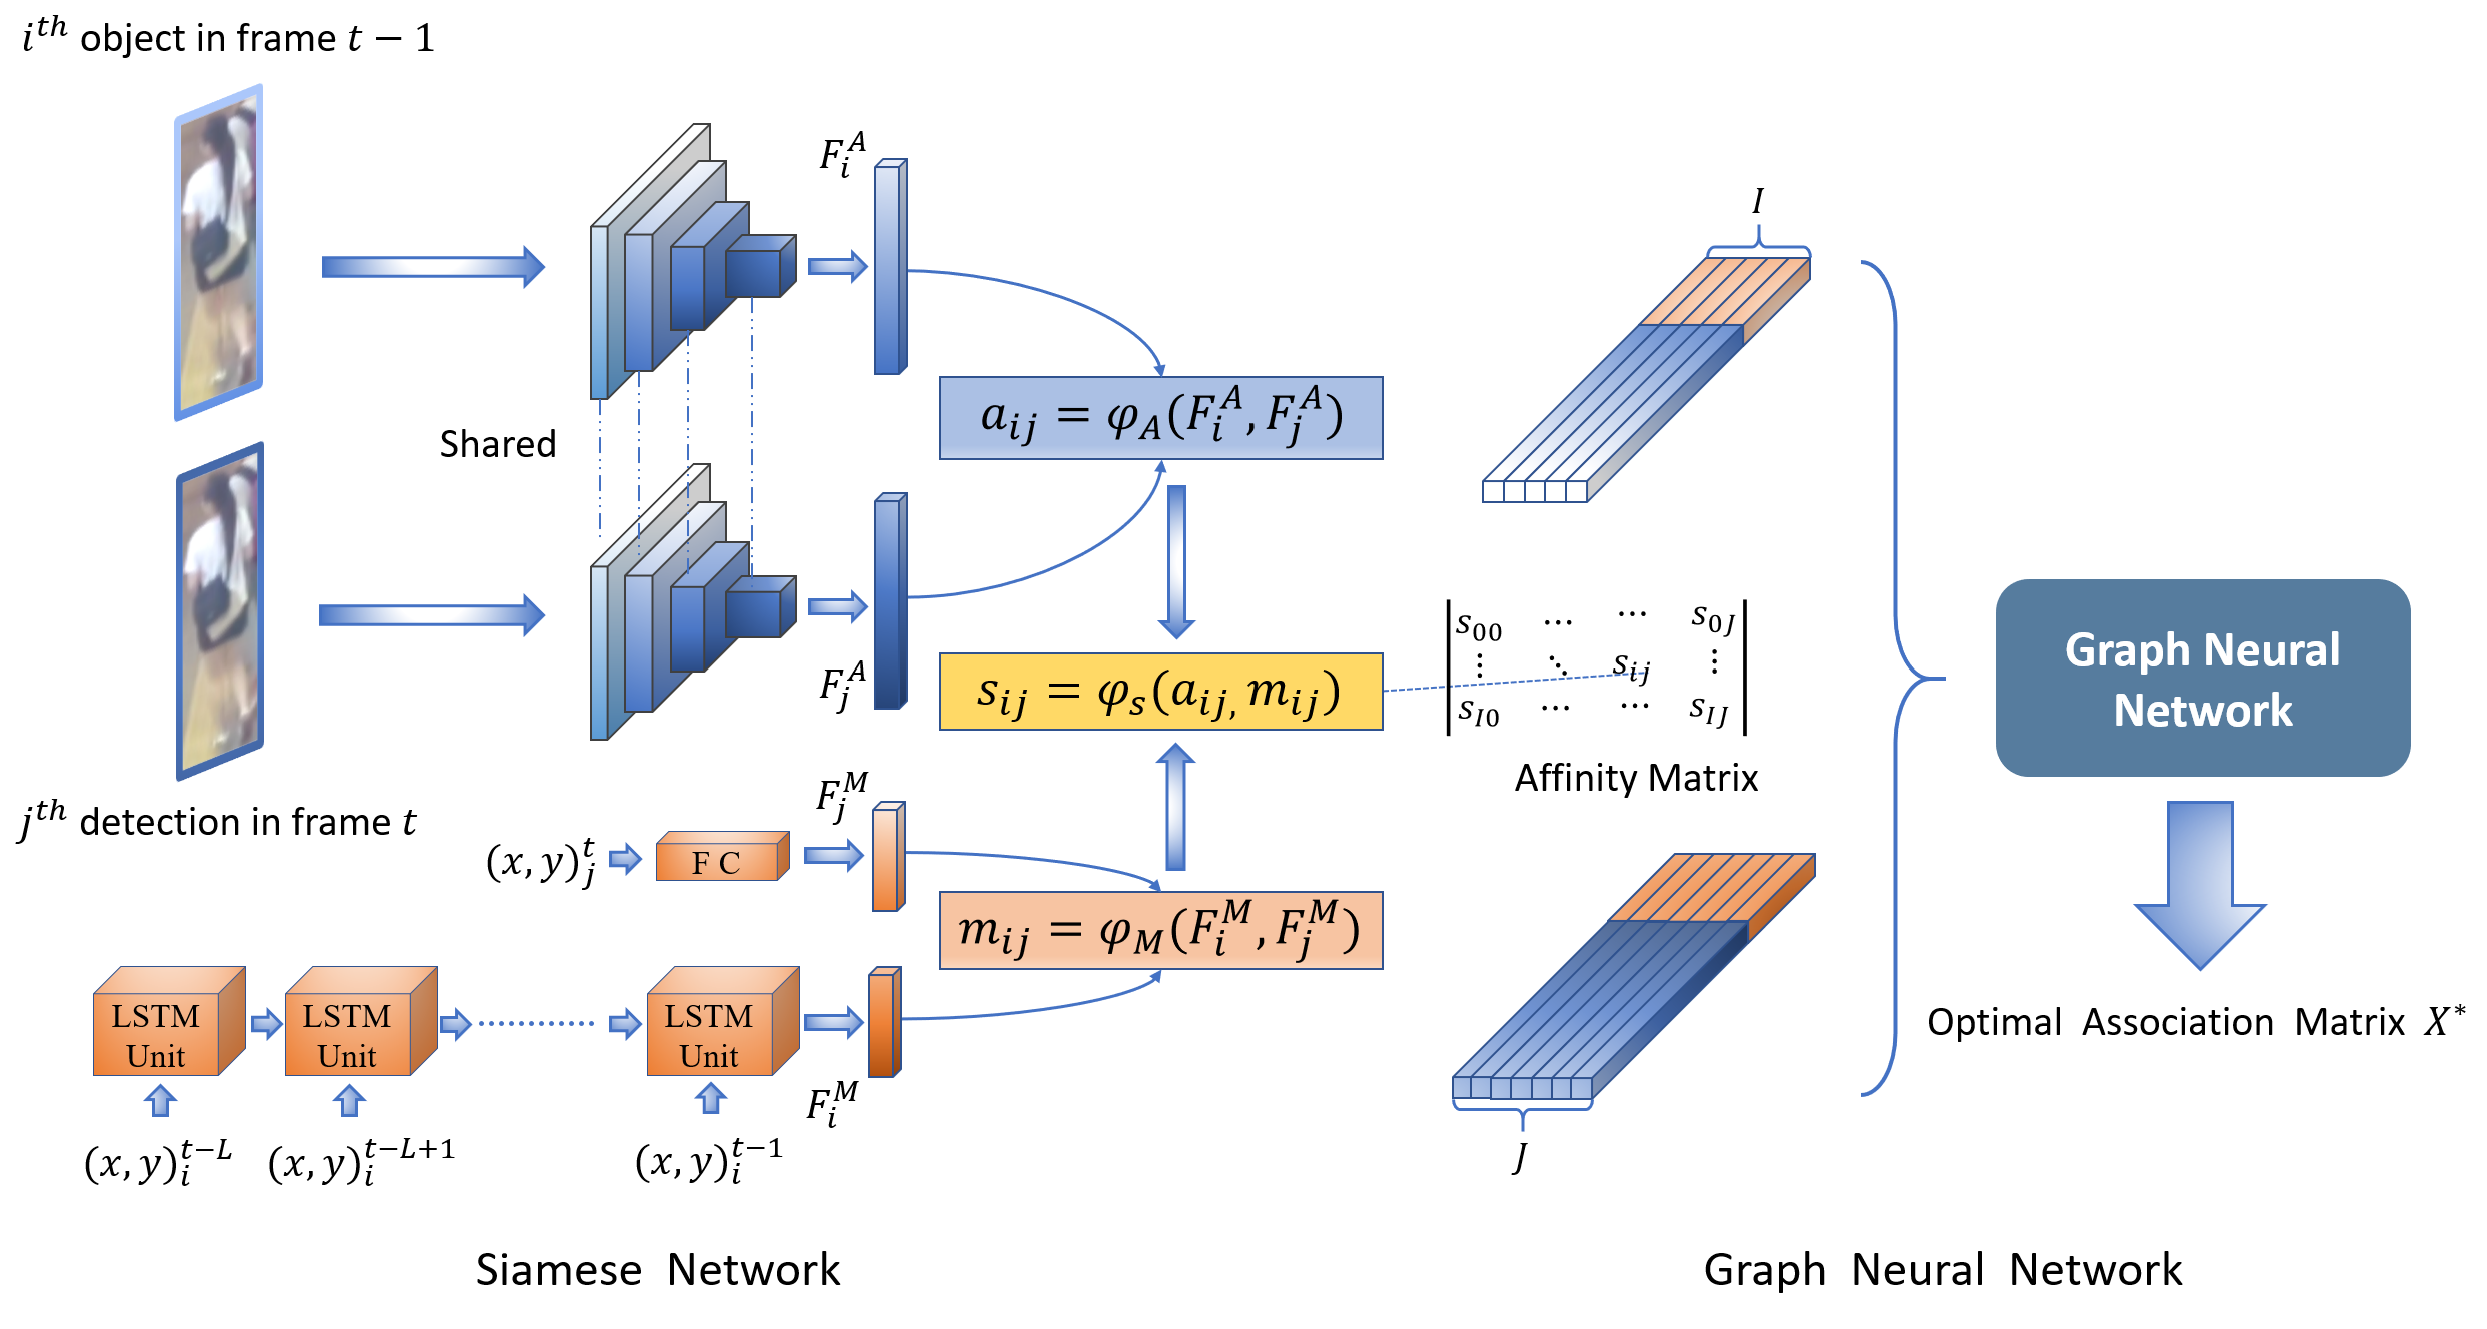
\includegraphics[width=5.4in]{imgs/pipeline.pdf}
	\caption{
		{An illustration to the framework of our Joint Detection Association Network (JDAN), which consists of three submodules: \emph{detection submodule} $S_D$, \emph{joint submodule} $S_J$, and \emph{association submodule} $S_A$.} 
%		A pair of video frames separated by $n$ time stamps $F_t$, $F_{t-n}$ are inputted to the network without pre-identified targets. 
%		The two input video frames are disposed of the two-stream detection network with shared parameters, where each stream forms an \emph{detection submodule} to learn robust and high-resolution object representations. 
		%
%		The number in the backbone network indicates the stride, 
%		and we append positioning and representation heads for predicting object bounding boxes and detection representations $R_t$.
%		Then, $R_t$ and $R_{t-n}$ are copied $N_m$ times along the vertical and horizontal directions, respectively, to form $M_t \in \mathbb R^{128 \times N_m \times N_m}$ and $M_{t-n} \in \mathbb R^{128 \times N_m \times N_m}$. 
%		Complete combinations of these representation tensors $M_t$ and $M_{t-n}$ are concatenated into a \emph{confusion tensor} $M_{t-n,t} \in \mathbb R^{(128+128) \times N_m \times N_m}$. 
%		Subsequently, the $M_{t-n,t}$ is converted to an \emph{association matrix} $M_a \in \mathbb R^{N_m \times N_m}$ through an \emph{association predictor}. 
%		At the same time, the matrix is utilized to perform \emph{online} MOT by reviewing the historical video frames. 
	}
	\label{fig:pipeline}
\end{figure*}

\subsection{Detection Submodule} \label{sec:detection_submodule}
% tracking objects as points; 3; CenterNet takes
{
Given an input frame $F \in \mathbb{R} ^ {W \times H \times 3}$, where $W$ and $H$ are the width and height respectively, the \emph{detection submodule} generates several} object bounding boxes and their corresponding representations. 
%The \emph{detection submodule} takes a single video frame $F \in \mathbb{R} ^ {W \times H \times 3}$ as the input and gains the
%object bounding boxes and corresponding representations for each video frame. 
% fairmot, 3.2, Following, we treat object
% We consider detection submodule as a center-based bounding box regression problem on center point from a different resolution feature following~\cite{point}. 
In {our model}, two types of predictive heads are added to the backbone, 
{where} the \emph{positioning head} locates target bounding boxes, 
% dan 3.2, The resulting processed
{and} the \emph{representation head} generates object representations.
{
Next, we will elaborate the backbone and the two heads.
}
%, presented in Fig.~\ref{fig:pipeline},  
% dan 3.2, We model the
%and we input it to the latter part of the JDAN to obtain the \emph{association matrix} $M_a$ for each pair of video frames. 


%\begin{figure}
%	\centering
%	\includegraphics[width=3.6in]{imgs/detection.pdf}
%	\caption{
%		Detailed information of the \emph{Detection Submodule} in Fig.\ref{fig:pipeline}. 
%		We input the video frame $\boldsymbol{F}_t$ to an backbone network to learn a high-resolution object representation. 
%		The number in the backbone network indicate the stride, 
%		and we append positioning and representation heads for predicting object boxes and detection representations $\boldsymbol{R}_t$.
%		The $\boldsymbol{R}_t$ is learned for the \emph{association submodule} as depicted in Sec.\ref{sec:association_submodule}.
%	}
%	\label{fig:detection}
%\end{figure}


\subsubsection{Backbone Network} \label{sec:backbone}
% fairmot, 1 (2) Multi-layer feature
The backbone network is crucial for MOT task since 
{both low-resolution and high-resolution representations are necessary to be exploited for fitting} tracked targets on various scales. 
{
In our work, we use ResNet-34~\cite{resnet} as the backbone network to strike a balance between model complexity and precision.
In order to extract robust object representations, we introduce a variant of DLA~\cite{point} (deep layer aggregation) into ResNet-34.
Compared with the raw DLA~\cite{dla}, the variant of DLA has additional bypasses between the low and high layer representations,
and thus has stronger ability to handle various complex environments.
It is demonstrated that the variant of DLA is beneficial to alleviate the identity switch problem for one-stage approaches because the encoder-decoder network could deal with objects of varied sizes~\cite{point,fairmot}.
Moreover, all the convolutional blocks in upsampling process are displaced by the deformable convolutional module which can adaptively accommodate the change of target size~\cite{deformable,zhou2020tracking}.
%Based on the backbone, we append the positioning and representation heads for predicting object bounding boxes and detection representations.
%All the modifications above are likewise beneficial to extract  more refined object features~\cite{point,zhou2020tracking}. 
}


%The backbone network is crucial for MOT task since object representations require exploiting both low-resolution and high-resolution representations to fit tracked targets on various scales. 
% reinforced power
%FairMOT~\cite{fairmot} notices that deep layer aggregation (DLA) is beneficial to decrease \emph{ID\_Sw} for the one-stage approaches because the encoder-decoder network can deal with varied object sizes. 
%However, the DLA is not important in the two-stage approaches since bounding boxes will have the same size by clipping and scaling. 

% In our study, we use DLA as the backbone of the \emph{detection submodule}. 
% fairmot, 3.1, We adopt the ResNet
%In our study, to consider both model complexity and precision, ResNet-34~\cite{resnet} is employed. 
%We utilize a variant of DLA~\cite{point} as the backbone of the \emph{detection submodule} to adapt the target of various scales, as presented in Fig.~\ref{fig:pipeline}. 
%Compared with the raw DLA~\cite{dla}, it has additional bypasses between the low and high layer representations. 
%In addition, all convolutional blocks in the upsampling process are displaced by the deformable convolutional module~\cite{deformable} because it can adaptively accommodate the target size changes. 
%{These modifications are likewise beneficial to relieve the alignment problem~\cite{point,zhou2020tracking}.
%The number in the backbone network indicates the stride, 
%and we append positioning and representation heads for predicting object bounding boxes and detection representations.
%} 
% Indicate the scale of the model input as $H_{\text{img}} \times W_{\text{img}} \times 3$, 
% and the output of DLA has the size of $H \times W \times C$ where $H = \frac{H_{\text{img}}}{S} $, $W = \frac{W_{\text{img}}}{S} $, where downsampling factor $S=4$.


\subsubsection{Positioning Head} \label{sec:detection_head}
% fairmot, 3.2, Following; Each head 
{
The \emph{positioning head} generates location and size information by using three heads: \emph{heatmap head}, \emph{size head} and \emph{displacement head}. 
}

%The input of the \emph{positioning head} is the output representations of the backbone network. 
%Each \emph{positioning head} has a $3\times3$ kernel size and $256$ output channels, followed by a $1\times1$ convolution that produces the positioning output. 
%Specifically, it generates a low-resolution headmap and size map. 

% fairmot, 3,2; Heatmap Head; This head
The \emph{heatmap head} {aims} to predict an object center {for each object where we use $1$ to indicate the center and the smaller values in the range $(0,1)$ to represent the distance to the center.}
Given a bounding box $\boldsymbol{b}^i = (x_1^i,y_1^i,x_2^i,y_2^i)$ in the ground truth, we obtain the corresponding center position $ \boldsymbol{p}^i  = (\frac{x_1^i+x_2^i}{2}, \frac{y_1^i+y_2^i}{2})$.
{
Considering the downsampling operation, we use $\boldsymbol{q}^i = \lfloor \frac{\boldsymbol{p}^i}{G}  \rfloor $ to represent the center position on the representation map, where $G$ is downsampling factor.
The heatmap response at the center is set to $1$, and $r_{q} =  \mathrm{exp}^{-\frac{(\boldsymbol{q} - \boldsymbol{q}^i)^2}{2\sigma ^2}}  $
} at other positions, 
where $\sigma$ is the Gaussian kernel that is a function of target size~\cite{cornernet}. 
{
Given a predicted heatmap response 
}
$\hat{r}_{q} \in [0,1]^{\frac{W}{G} \times \frac{H}{G} }$, the heatmap loss function is formulated according to the focal loss~\cite{lin2017focal} as follows:
\begin{align}
\mathcal{L}_{h} = -\frac{1}{N} \sum _{q} \begin{cases} (1-\hat{r}_{q})^\alpha \text{log}(\hat{r}_{q}), & \text{if } r_{q}=1, \\ (\hat{r}_{p})^\alpha \text{log}(1-\hat{r}_{q}) (1-r_{q})^\beta & \text{otherwise,}
\end{cases}
\end{align}
where $N$ indicates the number of targets in the current video frame, and $\alpha,\beta$ are the hyperparameters of the focal loss. 
 

%The output of this head at a certain position is $1$ when it overlaps with the truly central target position. 
%The output value decreases as the distance to the central position of the target increases~\cite{cornernet}. 
%% modified by: Tracking Objects as Points
%For a ground truth bounding box $b^i = (x_1^i,y_1^i,x_2^i,y_2^i)$ in the video frame, we obtain the central position 
%$ p^i  = (\frac{x_1^i+x_2^i}{2}, \frac{y_1^i+y_2^i}{2})$ of the target. 
%Therefore, the position on the representation map is computed by dividing the central position by the downsampling factor 
%$q^i = \lfloor \frac{p^i}{G}  \rfloor $, where $G=4$. 
%% $\tilde{p}_i = (\tilde{p}_x^i, \tilde{p}_y^i) = (\lfloor \frac{p_x^i}{S} \rfloor, \lfloor \frac{p_y^i}{S} \rfloor)$, where $S=4$. 
%Formally, the heatmap response at the position $q \in \mathbb{R}^2$ is defined as 
%$r_{q} = \mathop{max}\limits_{i} ( \mathrm{exp}^{-\frac{(q - q^i)^2}{2\sigma ^2}} ) $, 
%% where $N$ is the number of targets in the current video frame
%where $\sigma$ is the Gaussian kernel that is a function of the target size~\cite{cornernet}. 
%% ???????????https://www.cnblogs.com/king-lps/p/9497836.html
%The heatmap loss function is formed as a training objective according to the focal loss~\cite{lin2017focal}: 
%\begin{align}
%\mathcal{L}_{h} = -\frac{1}{N} \sum _{q} \begin{cases} (1-\hat{r}_{q})^\alpha \text{log}(\hat{r}_{q}), & \text{if } r_{q}=1 \\ (\hat{r}_{p})^\alpha \text{log}(1-\hat{r}_{q}) (1-r_{q})^\beta & \text{otherwise}
%\end{cases}
%\end{align}
%where $N$ indicates the number of targets in the current video frame, $\hat{r}_{q} \in [0,1]^{\frac{W}{G} \times \frac{H}{G} \times C_h}$ is the predicted heatmap response at location $q$, and the class numbers $C_h=1$ and $\alpha,\beta$ are the hyperparameters of the focal loss. 

% fairmot, 3.2; Box Size Head
The \emph{size head} is used for predicting the width and height of an object around its central position, 
% fairmot; 3.2; Center Offset Head; This head is
{which} is defined as $\hat{Z} \in \mathbb{R}^{\frac{W}{G} \times \frac{H}{G} }$. 
% Box Size Head; This head is not
%Although the positioning accuracy is not directly correlated to the object representations, it will affect the performance of the detection subtask. 
% fairmot; 3.4; Offset; For each GT box
{Given} a ground truth box $\boldsymbol{b}^i$, the box size $\boldsymbol{z}^i$ is calculated as $(x_2^i-x_1^i, y_2^i-y_1^i)$, 
and the predicted bounding box size is noted as ${\hat{\boldsymbol{z}}}^i$. 
% \subsubsection{Center Offset and Box Size Head}
% fairmot; 3.3; Center Offset Head; We find
{
Moreover, as the downsampling operation will produce strong quantitative bias, we use the \emph{displacement head} to solve this problem, which is important for improving the accuracy of data association~\cite{fairmot}. 
} 
{Let} ${\hat{\boldsymbol{d}}}^i$ be the predicted box displacement, $\boldsymbol{d}^i$ denotes the corresponding ground truth which is calculated as $\boldsymbol{d}^i = \frac{\boldsymbol{p}^i}{G} - \lfloor \frac{\boldsymbol{p}^i}{G} \rfloor $, we employ the $L_1$ loss for \emph{size} and \emph{displacement heads} as follows:
\begin{equation}
\mathcal{L}_{s} = \frac{1}{N} \sum_{i=1}^{N} \|\boldsymbol{z}^i - \hat{\boldsymbol{z}}^i\|_1 + 
\frac{1}{N} \sum_{i=1}^{N} \|\boldsymbol{d}^i - \hat{\boldsymbol{d}}^i\|_1.
\end{equation}

%FairMOT~\cite{fairmot} demonstrates that the refined bounding box with a central position is importantn for improving the MOT precision. 
%% fairmot; 3.3; Center Offset Head; Recall that
%The downsampling factor $G$ in the backbone network will exert strong quantitative effects. 
%The \emph{displacement head} is utilized for detecting the targets more accurately. 
%Although the advantages for detection precision increase are negligible, 
%the \emph{displacement head} is import for MOT data association because the object representations are learned based on the extremely precise bounding boxes. 
%% fairmot; Offset and Size Loss
%We indicate the output of the \emph{displacement head} as $\hat{D} \in \mathbb{R}^{\frac{W}{G} \times \frac{H}{G} \times C_d}$, where the class number $C_d=2$. 
%The ground truth displacement on the representation map is also obtained through 
%$d^i = \frac{p^i}{G} - \lfloor \frac{p^i}{G} \rfloor $. 
%% $d^i = (\frac{c_x^i}{S}, \frac{c_y^i}{S}) - (\lfloor \frac{c_x^i}{S} \rfloor, \lfloor \frac{c_y^i}{S} \rfloor)$. 
%We indicate the central position displacement as ${\hat{d}}^i$. 
%Thus, we denote the analogous $L_1$ loss for \emph{size head} and \emph{displacement head}: 
%\begin{equation}
%\mathcal{L}_{s} = \frac{1}{N} \sum_{i=1}^{N} \|z^i - \hat{z}^i\|_1 + 
%\frac{1}{N} \sum_{i=1}^{N} \|d^i - \hat{d}^i\|_1.
%\end{equation}

{Finally,} the \emph{positioning loss} $\mathcal{L}_{p}$ is {formulated} as an assembly of the previous two losses:
\begin{equation} \label{equ:position_loss}
\mathcal{L}_{p} = \mathcal{L}_{h} + \mathcal{L}_{s}.
\end{equation}

\subsubsection{Representation Head}
% fairmot; 3.3; The goal
{T}he \emph{representation head} {aims} to extract object representations that can differentiate various tracked targets. 
{
Given a representation map $E \in \mathbb{R}^{\frac{W}{S} \times \frac{H}{S} \times C_e}$ by the backbone, where $S$ represents the scale and $C_e$ indicates the number of channels, 
the \emph{representation head} adopts the heatmap approach to generate an object representation $E_{p} \in \mathbb{R}^{C}$ for each target at the central $p$.
To better learn discriminative features for different objects, our approach designs an identity classification loss based on identity representation $E_{p}$ as follows: 
\begin{equation} \label{equ:classification_loss}
\mathcal{L}_{c} = - \frac{1}{N \times J} \sum_{i=1}^{N} \sum_{j=1}^{J} u^i{(j)} \text{log}(v(j)),
\end{equation}
where $j$ represents the identity index, 
and $i$ records the instance index of each identity. 
$v(j)$ is the classification probability for the identity $j$. 
$u^i(j)$ is the ground truth for the identity $j$. 
}
$J$ is the total number of identities {and $N$ is the instance number of each identity}. 
%In an ideal case, the differences between different pedestrians are greater than those between the same pedestrian. 
%To achieve this goal, an object representation is learned for a detected target on the basis of the backbone network output. 
%The generated representation map is $E \in \mathbb{R}^{\frac{W}{S} \times \frac{H}{S} \times C_e}$, where the output channel $C_e=128$. 
%The representation $E_{p} \in \mathbb{R}^{C}$ of a target at the central position $p$ is learned through the \emph{representation head}. 
% 3.4; Ientity; We treat
%We consider tracked target recognition as a classification problem. 
%In particular, all targets of the same identity in the training dataset are regarded as one label. 
%For a true box $b^i$ in a video frame, we obtain the target central position $\hat{p}^i$ on the heatmap. 
%We learn an identity representation $E_{p^i}$ at a certain position and output to a one-dimensional classification probability vector $v(k)$, 
%and denote the ground truth classification tag as $u^i{(j)}$. 
%Therefore, the identity classification loss is constructed as:
%\begin{equation}
%{
%\mathcal{L}_{c} = - \frac{1}{N \times J} \sum_{i=1}^{N} \sum_{j=1}^{J} u^i{(j)} \text{log}(v(j)),
%}
%\end{equation}
%where $J$ is the number of all identities in a dataset. 

Finally, the total \emph{detection loss} $\mathcal{L}_{d}$ is formed as an assembly of Equation~\ref{equ:position_loss} and \ref{equ:classification_loss}:
\begin{equation}
\mathcal{L}_{d} = \mathcal{L}_{p} + \mathcal{L}_{c}.
\end{equation}

% DAN 3.2 Deep Affinity Network

\subsection{Joint Submodule}

% dan; 3.2; We model: The DAN training
%The JDAN training needs the current frame $F_t$ and the historical frame $F_{t-n}$ without object bounding boxes as the network input. 
%In addition, JDAN needs a true \emph{binary association matrix} $B_{t-n, t}$ between the historical frame and current frame as a real label to compute the association loss (Depicted in Sec.~\ref{sec:similarity_loss}) in the training of the \emph{association submodule} $S_A$. 
%A pair of frames to JDAN is indicated on the far left in Fig.~\ref{fig:pipeline}. 
%We depict the details of the \emph{joint submodule}, the training process of the proposed JDAN and some data augmentation strategies. 

{
The \emph{joint submodule} connects \emph{detection} and \emph{association submodules}, and aims to generate a \emph{confusion tensor} for paired frames.
Concretely, given}
two representations $R_t \in \mathbb{R}^{128 \times N_m}$ and $R_{t-n} \in \mathbb{R}^{128 \times N_m}$ (the position of placeholder object is filled with zeros), where $N_m$ is the max number of targets in a frame, 
{
our approach first copies $R_t$ with $N_m$ times
} along the vertical direction to construct a tensor $M_t \in \mathbb{R}^{128 \times N_m \times N_m}$, as well as copies $R_{t-n}$ $N_m$ times along the horizontal direction to generate a tensor $M_{t-n} \in \mathbb{R}^{128 \times N_m \times N_m}$.
{
Then, both $M_t$ and $M_{t-n}$ 
}
are merged along the channel direction to output a \emph{confusion tensor} $M_{t-n,t} \in \mathbb{R}^{(128 + 128) \times N_m \times N_m}$, 
{
which contains all the representation pairs of any two objects from the two frames.
Therefore, it offers all the object pairs for the next \emph{association submodule} to generate an \emph{association matrix} for MOT.
}

{
In the \emph{joint submodule}, all the object representations $R_t$, $R_{t-n}$ come from the \emph{detection submodule}, and may have data inconsistency with the tracking ground truth on MOT benchmark datasets.
Therefore, it is difficult to implement an \emph{end-to-end} training. 
To solve this problem, we discard the tracking ground truth, and adopt a simple yet effective traditional association method called Kalman Filter~\cite{welch1995introduction} to predict the locations of tracklets, resulting in tracking pseudo labels for the object representations $R_t$, $R_{t-n}$.
According to the pseudo labels, we obtain a pseudo \emph{association matrix} $B_{t-n,t} \in \mathbb{R}^{(N_m+1) \times (N_m+1)}$, where each element $b_{k,l}$ indicates the matching relationship between the object $k$ and $l$, and the added one column/row (noted as "+1" for $B_{t-n,t}$) represents object disappearance/appearance in the current frame.
We define three values for $b_{k,l}$: $1$ indicates the same identity between the object $k$ and $l$ (called "pseudo positive pairs"), $0$ represents different ones (called "pseudo negative pairs"), and $0.5$ means uncertain.
In the implementation, we set a high threshold in Kalman Filter to reduce the false matching for pseudo positive pairs, and set a low threshold to increase the true mismatching for pseudo negative ones. The reamining pairs are set to uncertain.
%As a result, it generates a binary \emph{association matrix} $B_{t-n,t} \in \mathbb{R}^{(N_m+1) \times (N_m+1)}$, where $+1$ in column represents object disappearance in the current frame, and $+1$ in row indicates the object appearance in the current frame.
%Each element $b_{k,l}$ in $B_{t-n,t}$ represents the matching relation between object $k$ and $l$, where we use $1$ to indicate object $k$ and $l$ are the same identity, $0$ to be different ones, and $0.5$ to be uncertain.
%In the implementation, we set a high threshold in Kalman Filter to reduce the false matching between $k$ and $l$, and set a low threshold to increase the mismatching.
%The remaining pairs are set to uncertain.
}


%\subsubsection{Joint Submodule}
%{
%As depicted in Fig.~\ref{fig:pipeline}, there is \emph{joint submodule} $S_J$ between the object \emph{detection submodule} $S_D$ and \emph{association submodule} $S_A$.
%First, all object representations are concatenated to form representation matrices $R_t \in \mathbb{R}^{128 \times N_m}$ and $R_{t-n} \in \mathbb{R}^{128 \times N_m}$ (the position of placeholder object is filled with zeros), where $N_m$ is the number of upper limit targets in an input frame. 
%And our proposed \emph{joint submodule} $S_J$ copies the object representations $R_t$ in the current frame along the vertical direction to a tensor $M_t \in \mathbb{R}^{128 \times N_m \times N_m}$, 
%and copies the object representations $R_{t-n}$ in the historical frame along the horizontal direction to a tensor $M_{t-n} \in \mathbb{R}^{128 \times N_m \times N_m}$. 
%}
%Subsequently, the object representations $M_t$ and $M_{t-n}$ are merged along the channel direction of object representation to $M_{t-n,t} \in \mathbb{R}^{(128 + 128) \times N_m \times N_m}$, as illustrated in Fig.~\ref{fig:pipeline}. 
%We note that the vertical and horizontal copying is used to permute the two object groups as much as possible. 
%This ensures that a target in the historical frame $F_{t-n}$ possibly associates with all targets in the current frame $F_t$, and vice versa. 
%Then we transform the expanded \emph{confusion tensor} $M_{t,t-n}$ to an \emph{association matrix} $M_a \in R^{N_m \times N_m}$ through an \emph{association predictor} that contains five convolutional blocks~\cite{inception}. 
%Detailed information about the \emph{association predictor} is described in Table~\ref{tab:compression_net}. 
%{
%Thus, the \emph{association matrix} can be utilized to perform \emph{online} MOT by reviewing the historical video frames. 
%}


\begin{table}[t]
	\centering
	\tabcolsep=3.5pt
	\caption{A specification of the \emph{association predictor}. 
%		in Fig.
%	~\ref{fig:pipeline}:  
%		\emph{Input} is the number of the input channels in a convolutional module, 
%		\emph{Output} is the number of the output channels, 
%		$Kernel$ indicates $1 \times 1$ kernel to reduce dimension,
%		$Stride$ is the stride size,  
%		\emph{Stride} and \emph{Padding} are the same in both spatial dimensions. 
%		\emph{ReLU (Yes/No)} indicates whether the ReLU operation is utilized. 
%		\emph{BatchNorm (Yes/No)} indicates whether the batch normalization operation is utilized. 
	}
	\label{tab:compression_net}
	\centering
	\setlength{\tabcolsep}{3.5pt}
	\begin{tabular}{cccccccc}
		\hline
		\hline
		{Index} & {Input} & {Output} & {Kernel} & {Stride} & {Padding} & {ReLU} & {BatchNorm} \\
		\hline
		%\multirow{*}{}
		1     & 256  & 128  	& $1 \times 1$ 	& 1 & 0 &	Yes	&	Yes\\
		2     & 128   & 64   	& $1 \times 1$	& 1 & 0 &	Yes	&	Yes\\
		3     & 64   & 32   	& $1 \times 1$ 	& 1 & 0 &	Yes	&	Yes\\
		4     & 32   & 16   	& $1 \times 1$ 	& 1 & 0 &	Yes	&	No\\
		5    & 16    & 1    	& $1 \times 1$ 	& 1 & 0 &	Yes	&	No\\
		\hline
		\hline
	\end{tabular}%
\end{table}%

%\subsubsection{Jointing Consistency in Training Data}
%The ground truth bounding boxes in MOT benchmark datasets and the results of our \emph{detection submodule} are inconsistent, 
%and the corresponding detector implementation in MOT benchmark data that is necessary in \emph{end-to-end} MOT is unknown. 
%Therefore, we exploit the bounding boxes and identity trajectory information provided by the trained \emph{detection submodule} and the traditional association method in the MOT benchmark dataset to solve the problem of inconsistency of ground truth bounding boxes as depicted in Fig.~\ref{fig:consistency}. 
%
%
%{First, we use the pretrained \emph{detection submodule} and a traditional association method~\cite{welch1995introduction}, which utilize Kalman Filter to predict the locations of tracklets, to generate a series of trajectories in the MOT datasets.} 
%Then, these trajectory results are utilized to form a \emph{binary association matrix} $B_{t-n,t}$ following Sec.~\ref{sec:similarity_loss}, 
%that is then exploited to train the \emph{association submodule}. 
%Finally, we use a two-stage training strategy, as depicted in Sec.~\ref{sec:two_stage} to train the whole JDAN with consistent ground truth between the output of \emph{detection submodule} and the input of \emph{association submodule}. 




% label generation


% nongfu
\subsection{Association Submodule} \label{sec:association_submodule}
\label{sec:association_submodule}
% DAN??3.2.3, The objective 
{Given a \emph{confusion tensor} $M_{t-n,t}$,} \emph{association submodule} $S_A$ computes the association between two target groups in the frame $F_{t-n}$ and $F_t$.
%The aim of the object \emph{association submodule} $S_A$ in JDAN is to compute the associations between these two object groups in $F_{t-n}$ and $F_t$ with a concatenated \emph{confusion tensor} $M_{t-n,t}$. 
{
Table~\ref{tab:compression_net} demonstrates the structure of the \emph{association predictor},
which transforms the \emph{confusion tensor $M_{t-n,t}$} into an \emph{association matrix} $M_a \in \mathbb R^{N_m \times N_m}$, which records the association information between those inter-frame targets ($N_m$ is the max number of targets).
Concretely, the prediction implements the dimensionality compression from 256 to 1 step-by-step along the direction of object representation with a $1 \times 1$ kernel.
%For the association matrix $M_a \in \mathbb R^{N_m \times N_m}$, $N_m$ is the max number of objects.
Each row in $M_a$ represents a target in $F_{t-n}$, and each column indicates that in $F_{t}$.
The element $m_{k,l}$ in $M_a$ records the matching probability between the $k$-th target in $F_{t-n}$ and the $l$-th target in $F_t$. 
}

{
To deal with the object disappearance and appearance problems across frames, Fig.~\ref{fig:loss} illustrates the detailed process. 
Given an \emph{association matrix} $M_a$, we append a column to build $M_1 \in \mathbb R^{N_m \times (N_m + 1)}$, where the $m$-th row represents the $m$-th target in $F_{t-n}$ associated with $N_m+1$ targets in $F_t$,
and the new added column indicates these new targets appearing in $F_t$. 
In this way, we add an extra column to $M_a$, which is represented as ${\bf u} \in \mathbb R^{N_m} = \lambda {\bf 1} $, where $\lambda$ is a hyperparameter, and ${\bf 1}$ is an all-ones vector~\cite{dan}.
This design simulates the situation of target disappearance with a probability.
On this basis, we normalize the horizontal vector by performing a softmax function~\cite{train_mot}, resulting in the association probability matrix $A_1$ between all the targets in $F_{t-n}$ and $F_t$.
We delete the last column of $A_1$ to obtain the matrix $A_c$ with $N_m \times N_m$ dimension.
%$A_c$ and $A_r$ indicate that the matrices $A_1$ are clipped to the dimensions of $N_m \times N_m$ by deleting the last vertical vector and last horizontal vector, respectively, as depicted in Fig.~\ref{fig:loss}. 
Similarly, the target appearance is simulated by appending a row to build $ M_2 \in \mathbb R^{ (N_m + 1) \times N_m}$, $A_2 \in \mathbb R^{(N_m +1) \times N_m}$ and $A_r \in \mathbb R^{N_m \times N_m}$.
Finally, we utilize the \textit{max} function to obtain $A_m \in \mathbb R^{N_m \times N_m}$, which is the maximum of the corresponding position in both $A_c$ and $A_r$.
%the \textit{max} function also influences each element on its arguments. 
}

%Taking the target disappearance into consideration, we append an additional column to $M_a$ to build $M_1 \in \mathbb R^{N_m \times (N_m + 1)}$, as depicted at the top of Fig.~\ref{fig:loss}. 
%% dan; 3.2.3; network loss; In our
%The $m^{\text{th}}$ row of the expanded matrix $ M_{1}$ associates the $m^{\text{th}}$ object in frame $F_{t-n}$ with $N_m+1$ objects in frame $F_t$, where $+1$ indicates the undetected targets in the current frame $F_t$. 
%Moreover, we add an extra column and row to the object \emph{association matrix} $M_a$ to obtain understandable loss design. 
%The added vector for the \emph{association matrix} $M_a$ is ${\bf u} \in \mathbb R^{N_m} = \lambda {\bf 1} $, where $\lambda$ is a hyperparameter in the experiment, and ${\bf 1}$ is a unit vector consisting of ones only~\cite{dan}. 
%This design in the added vector means that all tracked objects have a probability of disappearance or appearance. 
%In addition, the \emph{pseudo association matrix} $B_{t-n,t}$ is implemented in the same manner. 
%Then, we normalize the expanded probabilistic vector in the horizontal direction of $ M_1$ by performing a softmax function~\cite{train_mot}. 
%Therefore, the horizontal vector of the output association matrix $A_{1} \in \mathbb R^{N_m \times (N_m +1 )}$ signifies association probabilities between all targets in video frame $F_{t-n}$ and all targets in video frame $F_t$, including the unidentified targets in the current video frame. 
%%
%Similarly, the target appearance is formed by appending an additional row to $M_a$ to build $ M_2 \in \mathbb R^{ (N_m + 1) \times N_m}$, as depicted at the bottom of Fig.~\ref{fig:loss}. 
%Then, we perform a vertical softmax function on $M_2$ to obtain $A_2 \in \mathbb R^{(N_m +1) \times N_m}$, whose column indicates the association probabilities from the video frame $F_{t-n}$ to $F_t$~\cite{train_mot}.





%\subsubsection{Association Predictor}
%\label{sec:similarity_estimator}
%% The architecture of
%The structure of the \emph{association predictor} is designed according to the practical meaning of $M_{t-n,t}$ and $M_a$, as depicted in Table~\ref{tab:compression_net}. 
%The module transforms the combination of target representations $M_{t-n,t}$ into an \emph{association matrix} $M_a$ that represents association information between these interframe-tracked targets~\cite{dan}. 
%Therefore, it implements dimensionality compression from $256$ to $1$ step-by-step along the direction of the object representation with a $1 \times 1$ kernel size. 
%% conducts cross-channel information exchange and
%It does not mutually influence the adjacent channels in the representation maps. 
%
%
%
%% dan 3.2, We model the
%\subsubsection{Association Matrix} \label{sec:association_matrix}
%We obtain the interframe associations by exploiting the proposed \emph{association submodule}, as depicted in the second half of Fig.~\ref{fig:pipeline},  
%% dan 3.2, The resulting, We compute
%and predict the object \emph{association matrix} $M_a$ between $F_{t-n}$ and $F_t$ by utilizing the largest number of targets $N_m$ permitted in each frame. 
%In this study, $N_m = 100$ is a sufficient upper limit for the MOT datasets, as explained in Sec.~\ref{sec:maximum_object}. 
%We insert zero vectors (as object placeholders) in the object similarity \emph{association matrix} $M_a$ along the horizontal and vertical directions following~\cite{dan} for generalization. 
%These zeros appear between $F_{t-n}$ and $F_t$ so that any video frame finally consists of $N_m$ targets and the shape of $M_a$ is $N_m \times N_m$. 

% Fig~\ref{fig:label} depicts the formation of $M_a$ used in the proposed method, where $N_m$ is set to $4$ to illustrate it. 
% The historical frame and the current frame have three pedestrians respectively, 
% and every video frame is responsible for four unique targets. 
%The row in $M_a$ indicates these objects in the historical frame,
%and the column indicates these objects in the current frame. 
%$M_a$ represents the medium matrix for the two video frames with horizontal and vertical object placeholders. 
%In $M_1$ and $M_2$, the medium matrix is appended with an additional horizontal and vertical vector at the end, known as \emph{unidentified} objects~\cite{dan}. 
%The appended vertical vector at the end is responsible for presently tracked objects that disappear from the historical frame $F_{t-n}$. 
%And the appended horizontal vector in the last row is responsible for emerging targets that come into the field of view in the current frame $F_t$, as depicted in Fig.~\ref{fig:loss}. 
%In particular, our proposed network can indicate multiple target disappearances and appearances in the field of view. 
%For example, we can replace 0 with 1 at multiple rows in the last appended vertical vector to indicate disappearance, 
%and replace 0 with 1 at multicolumn in the last appended horizontal vector to indicate appearance. 


\begin{figure*}[t]
	\centering
	\includegraphics[width=\textwidth]{imgs/loss.pdf}
	\caption{
		{The technical route of \emph{association submodule} in processing target disappearance and appearance}.
%		The process of object disappearance and appearance}. 
		For the input historical and current frames, we predict the similarity {\emph{association matrix}} $M_a$. 
		In consideration of multi-object disappearances and appearances between the historical and current video frames, $M_1$ and $M_2$ are designed by adding an additional column and row to $M_a$. 
		{Then, the horizontal and vertical softmax operations are conducted on $M_1$ and $M_2$ respectively, 
		and the cropped matrices $A_c, A_r$ are utilized to compute loss $\mathcal{L}_m$ by using the pseudo association labels.} 
		Finally, the total association loss $\mathcal{L}_s$ is constructed according to the sum of $\mathcal L_t$, $\mathcal L_m$ and $\mathcal L_b$. 
		% ($\boldsymbol{A}_a$ and $\boldsymbol{A}_b$). 
		% using $\boldsymbol{A}_c$ and $\boldsymbol{A}_r$
	}
	\label{fig:loss}
\end{figure*}

% 3.2.3? Network loss
%\subsubsection{Disappearance and Appearance} \label{sec:similarity_loss}
%% fairmot; 3.2.3; The architecture, For a moment
%% We compute the \emph{association matrix} $\boldsymbol{M}_a \in \mathbb R^{N_m \times N_m}$ via the \emph{association submodule}. 
%We can compute the network loss between inferred \emph{association matrix} $M_a$ and true \emph{binary association matrix} $B_{t-n,t} \in \mathbb{R}^{(N_m+1) \times (N_m+1)}$. 
%The label of the \emph{association matrix} is finally utilized to train the proposed \emph{association submodule} $S_A$. 
%Nevertheless, $M_a$ neglects the target disappearance and appearance between the historical and current frames. 
%Therefore, we utilize an encoding of similarity association between the historical frame and current frame to take multiple target disappearances and appearances into account. 

%Taking the target disappearance into consideration, we append an additional column to $M_a$ to build $M_1 \in \mathbb R^{N_m \times (N_m + 1)}$, as depicted at the top of Fig.\ref{fig:loss}. 
%% dan; 3.2.3; network loss; In our
%The $m^{\text{th}}$ row of the expanded matrix $ M_{1}$ associates the $m^{\text{th}}$ object in frame $F_{t-n}$ with $N_m+1$ objects in frame $F_t$, where $+1$ indicates the undetected targets in the current frame $F_t$.. 
%Then, we normalize the expanded probabilistic vector in the horizontal direction of $ M_1$ by performing a softmax function~\cite{train_mot}. 
%Therefore, the horizontal vector of the output association matrix $A_{1} \in \mathbb R^{N_m \times (N_m +1 )}$ signifies association probabilities between all targets in video frame $F_{t-n}$ and all targets in video frame $F_t$, including the unidentified targets in the current video frame. 
%%
%Similarly, the target appearance is formed by appending an additional row to $M_a$ to build $ M_2 \in \mathbb R^{ (N_m + 1) \times N_m}$, as depicted at the bottom of Fig.\ref{fig:loss}. 
%Then, we perform a vertical softmax function on $M_2$ to obtain $A_2 \in \mathbb R^{(N_m +1) \times N_m}$, whose column indicates the association probabilities from the video frame $F_{t-n}$ to $F_t$~\cite{train_mot}. 
%
%Moreover, we add an extra column and row to the object \emph{association matrix} $M_a$ to obtain understandable loss design. 
%The added vector for the \emph{association matrix} $M_a$ is ${\bf u} \in \mathbb R^{N_m} = \lambda {\bf 1} $, where $\lambda$ is a hyperparameter in the experiment, and ${\bf 1}$ is a unit vector consisting of ones only~\cite{dan}. 
%This design in the added vector means that all tracked objects have a probability of disappearance or appearance. 
%In addition, the \emph{binary association matrix} $B_{t-n,t}$ is implemented in the same manner. 

{
We design three loss functions to train the \emph{association submodule}.
The first one is called
}
\emph{direction loss} $\mathcal L_{d}$ which suppresses false target associations for disappearance and appearance as follows: 
%between the historical frame $\boldsymbol{F}_{t-n}$ to current frame $\boldsymbol{F}_t$, and $\boldsymbol{F}_t$ to $\boldsymbol{F}_{t-n}$. 
\begin{equation} \label{equ:direction_loss}
\mathcal L_t = \frac{\sum_{k=1}^{N_m} \sum_{l=1}^{N_m+1} \left( \left(-\log { A_1^{kl}} \right) \odot {B}_1^{kl} \right)}{ \sum_{k=1}^{N_m} \sum_{l=1}^{N_m+1} B_1^{kl} }  
+ \frac{ \sum_{k=1}^{N_m+1} \sum_{l=1}^{N_m} \left( \left(-\log { A_2^{kl}} \right) \odot {B}_2^{kl} \right)}{\sum_{k=1}^{N_m+1} \sum_{l=1}^{N_m} B_2^{kl}},
\end{equation}
% direction
where $B_1$ and $B_2$ are constructed by deleting the last row and column of $B_{t-n,t}$, respectively. 
The operator $\odot$ denotes the Hadamard product~\cite{hadamard}. 
%And all operations skip uncertain pseudo labels.
%{
%We skip the uncertain values when computing loss in this or latter.
%}
%In the direction loss, instead of forcing $A_q$ to fit ground truth association label $\boldsymbol{L}_q$ by utilizing a distance criterion, we optimize the probabilities presented by the related values in $\boldsymbol{A}_q$? where $q \in \left\{1,2 \right\}$. 
%We think that this method is more reasonable than minimizing a distance between a ground truth binary matrix $\boldsymbol{L}_q$ and a predicted association matrix $\boldsymbol{A}_q$. 
%In addition, we utilize the \emph{non-maximum loss} and \emph{balance loss} to train the target \emph{association submodule~}~\cite{dan}. 
% non-maximum

{The second one called} \emph{non-maximum loss} $\mathcal L_{m}$ penalizes the non-maximum association in disappearance and appearance for association computation~\cite{dan} as follows: 
\begin{equation} \label{equ:non-maximum_loss}
\mathcal L_m = \frac{ \sum_{k=1}^{N_m} \sum_{l=1}^{N_m} \left( \left(-\log A_m^{kl} \right) \odot {B}_3^{kl} \right)}{\sum_{k=1}^{N_m} \sum_{l=1}^{N_m} B_3^{kl}},
\end{equation}
where $B_3$ is defined by deleting both the last row and column of $B_{t-n,t}$. 
%$A_m = \max (A_c, A_r)$. 
%The \textit{max} function also influences each element on its arguments. 
%The $max$ operation is utilized in the design of loss $L_m$ to obtain the maximum in $A_c$ and $A_r$, 
%where $A_c$ and $A_r$ indicate that the matrices $A_1$ and $ A_2$ are clipped to the dimensions of $N_m \times N_m$ by deleting the last vertical vector and last horizontal vector, respectively, as depicted in Fig.~\ref{fig:loss}. 
{The third one called} \emph{balance loss} $\mathcal L_b$ penalizes any imbalance between disappearance and appearance branches, 
which means that the number of targets that appear and disappear from the field of view should be equal.
%which means that the matching probabilities in two branches should be equal.
%the number of objects appearing and disappearing are equal: 
\begin{equation} \label{equ:balance_loss}
\mathcal L_b =  \sum_{k=1}^{N_m} \sum_{l=1}^{N_m} \lvert A_c^{kl} - A_r^{kl} \rvert. 
% \mathcal L_b = \sqrt{ \sum_{i=1}^{N_m} \sum_{j=1}^{N_m} (\boldsymbol{A}_c^{ij} - \boldsymbol{A}_r^{ij} )^2 },
\end{equation}
%In addition, given the tiny difference between $A_c$ and $A_r$, the Manhattan distance is used to compute the \emph{balance loss} $\mathcal L_b$. 

Finally, the total association loss $\mathcal L_s$ is the sum of Equation~\ref{equ:direction_loss}, \ref{equ:non-maximum_loss} and \ref{equ:balance_loss}{:} 
\begin{equation} \label{equ:association_loss}
\mathcal L_{s} = \mathcal L_t + \mathcal L_m + \mathcal L_b{.}
\end{equation} 

{
%log} function {applies to the each element of input matrix. 
In the implementation, we only calculate pseudo positive and pseudo negative pairs, and discard uncertain pairs for the three losses.
}
%Here, the training aim of the \emph{association submodule} is to minimize the association loss $\mathcal{L}_s$. 
%{Therefore, the three losses above are effective and lead to a fitting of the pseudo-labelling object association.} 


\subsection{Training and Testing}
%In this part, we describe the {training strategy,} the usage of the proposed \emph{end-to-end} network and the detailed steps for performing MOT in video frames without input bounding boxes. 

\subsubsection{{End-to-end Training}} \label{sec:two_stage}
% DAN, 3.2, To align
JDAN contains two trainable submodules: \emph{detection submodule} $S_D$ and \emph{association submodule} $S_A$.
{
Our approach adopts an iterative training process to train the model which consists of two steps:
First, we adopt a pretrained object detection model on several detection datasets~\cite{zhang2017citypersons,ess2008mobile,xiao2017joint,dollar2009pedestrian,zheng2017person} and fine-tune its parameters according to the detection loss $\mathcal{L}_{d}$ on the basis of ground truth; 
Second, given the pseudo labels on detected targets by utilizing Kalman Filter~\cite{welch1995introduction}, 
we update both \emph{detection} and \emph{association submodules} according to $\mathcal{L}_{s}$ in Equation~\ref{equ:association_loss}.
We iteratively repeat the above two steps until the loss $\mathcal{L}_{s}$ is converged.
Compared to the previous approaches, errors could be propagated back to update both \emph{detection} and \emph{association submodules},
and thus our approach could achieve an \emph{end-to-end} training to alleviate the error propagation problem.
}
%{The proposed} JDAN contains two trainable submodules, named the \emph{detection submodule} $S_D$ and \emph{association submodule} $S_A$. 
%%Finally we perform an \emph{end-to-end} inference. 
%First, both ground truth boxes and identity information are utilized to train the \emph{positioning head} and \emph{representation head} using \emph{detection loss} $\mathcal{L}_{d}$, as depicted in Sec.~\ref{sec:detection_submodule}. 
%%While some data only have ground truth bounding boxes~\cite{zhang2017citypersons,ess2008mobile}, they are utilized to train the \emph{positioning head}.
%% as depicted in Sec.~\ref{sec:detection_submodule}. 
%{Second, we perform the traditional data association method~\cite{welch1995introduction,fairmot} on MOT datasets based on the bounding box generated by the pretrained \emph{detection submodule} $S_D$, 
%and utilize the output to generate the \emph{pseudo association matrix} $B_{t-n,t}$ as the pseudo-labels for training the \emph{association submodule} $S_A$ using association loss $\mathcal{L}_s$.
%Then, we repeat the first and second step of training until the loss has converged.
%}
%Due to the use of the pretrained \emph{detection submodule} and the online pseudo-labels, the generated object representations and association labels are consistent when training. 
%{
%Thus, these strategies ensure that the end-to-end training between detection and association can realize.
%}
%the bounding boxes and object representations generated by the \emph{detection submodule} are consistent between $S_D$ and $S_A$ in the second training stage. 
%{Finally, we can implement end-to-end training based on the previous pre-trained \emph{detection submodule} and \emph{association submodule}.}

%{Afterwards,} we fix the parameters of the \emph{detection submodule} $S_D$ to be consistent with the generated bounding boxes through $S_D$, 
%and train $S_A$ using the \emph{confusion tensor} produced by the \emph{joint submodule} $S_J$ and the \emph{binary association matrix} generated by the traditional data association method. 

%\label{sec:dep}
%\subsubsection{Model Prediction}
%% DAN, 3.3 Whereas the
%Although the object \emph{detection submodule} in JDAN is trained as two parallel branches, we only use a single network for \emph{online} MOT. 
%This is reasonable because the two parallel \emph{detection submodules} share their weights. 
%The inference of our proposed network is depicted by presenting the main modules in an orderly fashion in Fig.~\ref{fig:tracking}. 
%% FairMOT 3.5 Network Inference
%The input of the JDAN is a video frame $F_t$ with a shape of $1088 \times 608$ based on the previous study~\cite{jde}. 
%% FairMOT 3.5 Network Inference: On top
%Based on the inferred heatmap according to Sec~\ref{sec:detection_head}, a non-maximum suppression operation is conducted according to the heatmap responses to obtain the strongest points. 
%The positions of the points where the heatmap strongest responses exceed the limit value are selected. 
%Then, the corresponding boxes on the basis of the inferred size and offset are predicted. 
%Moreover, the object representations on the inferred central positions are learned, 
%and we use these object representations to perform data association between the current and historical frames in Sec~\ref{sec:association_submodule}.

% DAN 3.3 The feature extractor
%Moreover, the \emph{representation head} in \emph{detection submodule} learns the object representations $R_t$ and $R_{t-n}$ for the current and historical video frames. 
%%and delivers to the \emph{association predictor}. 
%The two representation matrices are copied and permuted to the \emph{confusion tensor} $M_{t-n,t}$ for these two images. 
%Then, the tensor $M_{t-n, t}$ is converted to an \emph{association matrix} $M_a$ by a common forward propagation through the \emph{association predictor}, as depicted in Sec.~\ref{sec:association_submodule}. 

\begin{figure}[t]
	\centering
	\includegraphics[width=5.3in]{imgs/tracking.pdf}
	\caption{
		Online MOT by JDAN. 
		Given an input video frame $F_t$, the target boxes and representations are supplied by the \emph{\emph{positioning} and \emph{representation heads}, respectively}, with a single stream \emph{detection submodule} in JDAN. 
		The object representation $R_t$ is used to pair with the latest $n$ historical representation $R_{t-n:t-1}$, 
		and every pair of representations is passed through the \emph{joint \& association submodules} to estimate the corresponding \emph{association matrix} $M_{t-n:t-1,t}$. 
		%For simplicity, here we set $\mu_m = t$. 
		In addition, the representation $R_t$ is reserved to estimate the \emph{association matrix} in the next $n$ frames. 
		Finally, we update the track recorder by linking the present image objects with $n$ historical image objects by utilizing the inferred \emph{association matrix}. 
	}
	\label{fig:tracking}
\end{figure}


% DAN 3.4, To associate
\subsubsection{Online Tracking}
% For the purpose of target association between the current image and multiple historical images, we record the sequential representation to carry temporal information. 


{
Fig.~\ref{fig:tracking} illustrates the \emph{online} tracking process by JDAN.
Given an input frame $F_t$, the \emph{detection submodule} predicts target representations $R_t$ for all the targets in $F_t$.
Then, the representation $R_t$ and historical representations $R_{t-n:t-1}$ are passed into the \emph{joint \& association submodules} to generate the corresponding \emph{association matrix} $M_{t-n:t-1,t}$, which are passed into the \emph{trajectory manager} to updates accumulator by using Kuhn-Munkres method~\cite{Munkres1957}. 
Concretely, tracks in \emph{trajectory manager} store tracking information for the historical frames $F_{t-n:t-1}$, 
and every element in accumulator is the sum of similarities of a track to the detected objects in the current frame. 
Here, a track corresponds to a target identity, and is a recorder of a key-value pair, where key is the index of a historical frame, and value is the corresponding target representation in that frame.
After receiving a new target representation $R_t$ in $F_t$, \emph{trajectory manager} would reserve the representation $R_t$ and output all the representations $R_{t-n:t-1}$, $R_t$ into the \emph{joint \& association submodules} to generate the \emph{association matrix} $M_{t-n:t-1,t}$ between each historical frame $F_{t-n}$ and the current frame $F_t$.
After that, the accumulator in \emph{trajectory manager} are updated, and the tracking results $T_t$ in $F_t$ are generated.
}
{
Some special cases have been considered in our method.
For instance, a historical track may has no matching target in the current frame, which indicates a target disappears.
In such case, we add a column in the acculumator to make each track corresponding to a sole column.
% 
The cost of \emph{online} tracking is composed of two parts: 
the \emph{detection submodule} to generate representation $R_t$ for the current frame, and the \emph{joint \& association submodules} to output tracking results $T_t$.
To ensure tracking speed, we adopt lightweight detection and association networks, and all the historical information including $R_{t-n:t-1}$ are stored in \emph{trajectory manager} without recalculation.
Therefore, our \emph{online} tracking could achieve a fast speed.
}



%After initializing the tracking process and generating $R_0$ in the first frame, we can infer an \emph{association matrix} between the current frame targets and those in a historical frame with the corresponding object representations. 
%The inferred \emph{association matrix} is utilized to refresh previous tracking results by reviewing the historical frame information, as depicted in Fig.~\ref{fig:tracking}. 



%Here, we describe the detailed \emph{online} tracking process shown below. 
%The recorder $T_0$ has the same number of tracks, as identified targets are initialized in the first video frame $F_0$. 
%In addition, every track is a recorder of key-value pairs, 
%and every item contains the video frame index and the target representation. 
%% ???????????? ?????
%We update the track recorder at the current frame using the Kuhn-Munkres method~\cite{Munkres1957}, 
%and realize it by maximizing the inferred associations between the present targets and the targets formerly associated with the trajectories in historical frames. 
%Additionally, we record it into an accumulator $Y_{t}$.
%%$Y_{t} \in \mathbb{R}^{{X}({T}_{t-1})\times{X}({T}_{t})}$, where $X$ is a function to evaluate the number of element for its input arguments. 
%% ?????????????????
%Every element in matrix $Y_{t}$ is the similarity summation of a target in the historical trajectory recorder $T_{t-1}$ to a target in the current frame. 
%The Kuhn-Munkres method deals with the maximum matching issue of a bipartite graph. 
%We form the issue using the accumulative matrix $\boldsymbol{Y}_{t}$.
% +1???????????
%In this, the row encodes the existing targets in the history frame,
%and the column represents these associations to the targets in the present video image. 

%The Kuhn-Munkres method gets matches between the current targets and these historical trajectories. 
%The process is realized by maximizing the similarities between the present targets and the targets formerly associated to the trajectories in historical images. 
%The utilized accumulative matrix encodes the similarities between targets in the current image and these in the historical images. 

% DAN 3.4, 3, At each
%For every video frame, we can estimate association matrices $M_a$ effectively with the proposed network to review the pre-existing trajectory information. 
%A minor problem for correctly utilizing the Kuhn-Munkres method to the MOT context is that it enables the tracked object to disappear between video frames. 
% ??????????

%Hence, a frame is transferred through the \emph{detection submodule} only once. 
%However, the object representations are utilized repeatedly many times to evaluate the similarities with the remaining images. 
% ???????????????
%many a track can be allocated to a particular undetected object column in the accumulative matrices based on the \emph{association matrix}. 
%This problem is solved by copying the last vertical vector of the accumulator until each track is allocated to a sole vertical vector~\cite{dan}. 
%Therefore, this strategy enables every undetected track to be associated with an undetected target. 

% DAN 3.4, 3, Overall ??
%In summary, the proposed detector-tracker is an \emph{online} MOT method that does not utilize any future information to infer target tracks. 
%Therefore, it can be applied to \emph{online} applications. 
%A potential problem is that an overlong trajectory may lead to large storage and computational costs. 
%Therefore, the threshold value $\mu_m$ is used to limit the number of frames that are reviewed in the existing trajectory. 
%The farthest object information is discarded if the number of images in a track exceeds $\mu_m$. 
%Moreover, if a tracked object disappears from the field of view for more than $\mu_r$ frames, it will be removed from the tracking list~\cite{train_mot}. 
%We employ these superparameters in the proposed MOT method for physical significance. 
%These hyperparameters can be altered based on the run-time memory and the limits of the computation resources. 


\section{EXPERIMENTS}
% DAN 4. Experiments, In this section
This section demonstrates the experiments by JDAN. 
We first introduce datasets and implementation details of our proposed JDAN, 
and then illustrate the experimental results as well as make a deep analysis. 

\subsection{Datasets and Metrics}
% fairMOT 4.1, Following

{
Our datasets consist of two components: detection datasets and MOT datasets.
We first adopt several detection datasets to} train our \emph{detection submodule}. 
In particular, CityPersons~\cite{zhang2017citypersons} and ETH~\cite{ess2008mobile} datasets merely supply bounding box information, 
and we use them to train the \emph{positioning head}. 
{Moreover, }CUHK~\cite{xiao2017joint}, Caltech~\cite{dollar2009pedestrian} and PRW~\cite{zheng2017person} could supply both pedestrian bounding box and identity information,
and thus we can train the \emph{positioning} and \emph{representation heads} jointly. 
%{Finally, we generate pseudo association labels to train the object \emph{association submodule} by performing the MOT process according to the result of trained \emph{detection submodule} and the traditional association method~\cite{kernelized,welch1995introduction}.} 
% FairMOT, 4.1, We extensively
For MOT task, we train and test our model on two benchmark datasets: MOT15~\cite{taix2015motchallenge} and MOT17~\cite{dendorfer2019cvpr19}. 
%The MOT17 contains seven training videos and seven test videos. 
{MOT15 consists of 11 training and 11 testing sequences with 5,783 frames, 61,440 bounding boxes and 721 tracks, 
while MOT17 contains 7 training and 7 testing videos with a longer duration including 17,757 frames, 564,228 bounding boxes and 2,355 tracks.}
%MOT17 consist of 7 training video and 7 test test videos.
%MOT16 consists of the same video sequences as the MOT17 dataset.
%We select the hyperparameters for our proposed model based on MOT17 benchmark dataset, which is chosen for hyperparameter adjustment because of its controllable scale. 
%And the inputs of JDAN are pure images without detection information. 
%% Performance Measures and a Data Set for Multi-Target, Multi-Camera Tracking
%Therefore, we only use the MOT17 dataset.

{For evaluation, we empoly a variety of metrics, including MOT accuracy (MOTA), MOT precision (MOTP), the ratio of correctly identified detection results to the mean number of the ground truth and predicted detection results (IDF1~\cite{ristani2016performance}), mostly tracked (MT) trajectories, mostly lost (ML) trajectories, identity switch (ID\_Sw), the total number of false positives (FP), the total number of missed targets (FN), the total number of fragmented trajectories (Frag)~\cite{clear}, and the number of frames processed per second (FPS).
Different metrics focus on different aspects to evaluate MOT performance.
}
%The evaluation metrics also include the ID\_Sw, ID Precision (IDP), the total number of false positives (FP), the total number of missed targets (FN), and the total number of fragmented trajectories (Frag)~\cite{clear}. 
% FairMOT, 4.1, We extensively, We use the
%We utilize these metrics on MOT benchmark to measure MOT performance. 


\subsection{Implementation Details} \label{sec:implementation_details}

% dan 4.1, We implement
{We} implement JDAN by using PyTorch 1.2.0~\cite{pytorch}, 
and the training process takes 20 hours on a Quadro RTX 6000 GPU. 
%Besides, the hyperparameters utilized in our experiment are described below. 
% fairmot, 4.2 The input image
%The proposed network has an input frame dimension of $1088\times608$. 
{
For each input frame, we first resize it to $1088\times608$, and then use}
a modification of DLA~\cite{point} in the \emph{detection submodule} as the backbone. 
{
As mentioned earlier, our training procedure consists of two steps.
}
% dan 4.1 All the training
%Prior to inputting it to the JDAN, these training and test samples are rescaled to the specified size. 
% fairmot 4.2; We use a 
First, we initialize the \emph{detection submodule} trained on Microsoft COCO~\cite{lin2014microsoft},
and adjust parameters with the SGD optimizer~\cite{sgd} for 50 epochs on detection datasets.
The initial learning rate is $1e-4$, and multiplied by 0.1 at the epochs 25 and 40. 
{
Second, we train the \emph{association submodule} with following settings:}
% The learning rate decreases to $1e-5$ and $1e-6$, at 25 and 40 epochs. 
% dan, 4.1, Batch size
the max number of objects $N_m$ in each frame is set to 100, the minibatch $B$ is set to 4, the training epoch is set to 160, and the multiplier of a unit vector $\lambda$ is set to 10. 
Moreover, we set the maximum gap $N_a$ between the historical and current frames to 30. 
Then, we train the whole model with the SGD optimizer~\cite{sgd}, where the momentum and weight decay are set to 0.9 and 5e-4, respectively. 
We launch the training with a learning rate of 0.01 that is multiplied by 0.1 at the epochs 60, 100 and 140. 

%In summary, the proposed detector-tracker is an \emph{online} MOT method that does not utilize any future information to infer target tracks. 
%Therefore, it can be applied to \emph{online} applications. 
{
A potential problem of an overlong trajectory may lead to a large storage and computational cost. 
Therefore, we set the threshold value $\mu_m$ to limit the number of frames that are reviewed in the existing trajectory, 
and the farthest target information is discarded if the number of images in a track exceeds $\mu_m=15$. 
Moreover, if a tracked object disappears for a duration of more than $\mu_r=12$ frames, it will be removed from the tracking list~\cite{train_mot}. 
We employ these superparameters in our approach for physical significance. 
%These hyperparameters can be altered based on the run-time memory and the limits of the computation resources. 
When the \emph{detection submodule} and \emph{association submodule} are trained,
% it is necessary to optimize $\mu_r$ and $\mu_m$. 
we choose the optimal values of the two hyperparameters with the grid search technique for the best MOTA performance on MOT training dataset.
% because of its controllable scale. 
We utilize multiples of three with the scope of $[3, 30]$ to construct the grid. 
%Thus, $\mu_m=15$ and $\mu_r=12$ are chosen with this approach in the real tracking process. 
}
% back, removed from the tracking list

%\subsubsection{{Data Augmentation}}
\label{sec:PP}
{In order to improve the accuracy, we exploit a series of data augmentation methods.
First,} we increase the frame size by using a random sampling rate in the range of 1.0-1.25, 
and fill the pixels in the expanded image with the average pixel value in MOT training set. 
% Cropping: 
{Second,} we clip the video frame randomly in the range of 0.75-1.0,
% Photometric distortions: 
and each pixel value in an image is multiplied by a value in the range of 0.75-1.25. 
The output frame is transformed to the $HSV$ space, 
and the saturation component is multiplied by a value in the range of 0.75-1.25. 
{Then,} the image is transformed back to the $RGB$ space and multiplied by a random factor sample~\cite{Liu2016}. 
%The input frame is scaled to $1088\times 608$, 
%and the size of the representation map is $272 \times 152$. 
%
{Besides,} we note that the historical frame $F_{t-n}$ and current frame $F_t$ are not necessarily consecutive in the video sequence,
and thus set them to be separated by $n$ frames, where $n \in [0, N_a-1] $. 
%However, the proposed JDAN is applied to associate the objects in successive frames. 
%Training using skipped frames is beneficial for the training of our proposed model between the current frame and those in a series of historical video frames. 
% 3.2.1 Multiple object tracking
%In addition, the training data~\cite{mot16,Lyu2017} utilized in MOT always lack the ability to capture the background variation, camera distortion and many realistic effects to maintain robustness in MOT. 
%In the proposed tracking method, it is vital that the training data involve involves enough uncorrelated tracking attributes to enhance the robustness of the MOT model. 
%Therefore, we carry out the subsequent data augmentation on the MOT training datasets. 
%
%
%% dan; 3.2.1; Each of the 
%All of the data augmentation methods are listed below, 
%We sample the historical and current video frames on every trajectory with a probability of 0.25. 
%Then, these video frames are reshaped to a specified size $W \times H \times 3$. 
%At the same time, only a horizontal flip with a probability of 0.5 is used. 
%The method for the modification of the MOT train set is inspired by~\cite{Liu2016} who modified video frames to enhance the training process. 
%Nevertheless, we synchronously dispose of historical and current frames using the previously reported data augmentation methods~\cite{Liu2016}. 

% 3.2.1 Multiple object tracking, Frame expansion




\subsection{Ablation {Studies}}
{
In order to prove the effectiveness of the proposed model, we conduct three ablation studies including the training paradigm, the representation dimension, and the maximum object number.
}

%\subsubsection{{Component Training}}

% FAMNet: Table 5
\begin{table}
	\begin{center}
		\caption{
		Ablative study with different training paradigms on MOT17 benchmark data. 
%			We present the optimum performance in {\bf bold}.
}
		\label{table:training_methods}
		\centering
		\setlength{\tabcolsep}{3.5pt}
		\begin{tabular}{c|c|c|c|c|c|c|c}
			\hline
			\hline
			Method & MOTA$\uparrow$ & MOTP$\uparrow$ & IDF1$\uparrow$ & MT$\uparrow$ & ML$\downarrow$ &  ID\_Sw$\downarrow$ & Frag$\downarrow$\\
			\hline
			{Baseline} & 20.7 & 38.3 & 38.2 & 17.6 & 48.8 & 24,875 & 6,731\\
			{Detection Training} & 34.6 & 42.8 & 40.4 & 19.9 & 46.7 & 18,264 & 4,084\\
			{Detection Fine-tuning} & {42.9} & {52.8} & {48.3} & {21.5} & {45.8} & {13,236} & {3,387}\\
			{Association Fine-tuning} & {53.0} & {65.2} & {49.7} & {23.4} & {44.3} & {11,875} & {2,845}\\
			JDAN & {\bf58.1} & {\bf79.8} & {\bf59.2} & {\bf27.7} & {\bf32.9} & {\bf6,129} & {\bf1,515}\\
			\hline
			\hline
		\end{tabular}
	\end{center}
\end{table}

% fairmot 4.3 Multi-Layer Feature Aggregation
\subsubsection{{Training Paradigm}}
In this stage, we evaluate the effect of several training processes by using our proposed components. 
As depicted in Table~\ref{table:training_methods}, we perform five ablations including {\emph{Baseline}, \emph{Detection Training}, \emph{Detection Fine-tuning}, \emph{Association Fine-tuning}} and JDAN. 
%The components of these methods are changed only once in each training method. 
% fairmot 4.3 Multi-Layer, We split
%We use MOT17 datasets to train the object \emph{association submodule}. 
%A large amount of data is not utilized here to validate the effectiveness of our training method. 
% fairmot: 4.3 Multi-Layer Feature Aggregation
%The tracking performance results are presented in Table~\ref{table:training_methods}. 
{
\emph{Baseline} first adopts a \emph{detection submodel} pre-trained on Microsoft COCO~\cite{lin2014microsoft}, and then uses an \emph{association submodule} fine-tuned with the generated pseudo labels.
On this basis, \emph{Detection Training} retrains the \emph{detection submodule} on the detection datasets, and then uses an \emph{association submodule} trained on the generated pseudo labels. 
Considering the visual gap between MOT and detection datasets, the third training paradigm called \emph{Detection Fine-tuning} employs a \emph{detection submodule} fine-tuned on MOT detection datasets to boost the detection performance,
%On the basis of \emph{Detection Training}, \emph{Detection Fine-tuning} uses a \emph{detection submodule} fine-tuned on MOT detection dataset.
while \emph{Association Fine-tuning} does not use MOT datasets for \emph{detection submodule} but fine-tunes \emph{association submodule} on MOT datasets.
%On the basis of \emph{Detection Fine-tuning}, \emph{Association Fine-tuning} uses a \emph{association submodule} fine-tuned on MOT association dataset.
%when fixing the parameter of \emph{detection submodule}. 
}
JDAN is the whole model fine-tuned on MOT datasets with an \emph{end-to-end} training for both \emph{detection} and \emph{association submodules}. 

{
Table~\ref{table:training_methods} reports the performance comparison results among the above training paradigms, and our analysis is list below: 
}
\begin{enumerate} 
\item Compared to \emph{Baseline}, \emph{Detection Training} achieves a significant performance improvement, with MOTA increasing from $20.7\%$ to $34.6\%$ and MOTP rising from $38.3\%$ to $42.8\%$.
This improvement indicates the effectiveness of retraining \emph{detection submodule} on the detection datasets since the pretraining on Microsoft COCO could not offer accurate pedestrian results for crowded scenes in MOT task.

\item {\emph{Detection Fine-tuning} further improves MOTA performance compared with \emph{Detection Training}}, with a significant improvement from $42.8\%$ to $52.8\%$ on MOTP, and from $18,264$ to $13,236$ on ID\_Sw. 
{
This improvement stems from the use of MOT datasets on \emph{detection submodule} to bridge the visual gap between the detection and MOT datasets.
Meanwhile, \emph{Association Fine-tuning} also achieves the same improvement as compared to \emph{Detection Fine-tuning} due to the use of MOT datasets to update the \emph{association submodule}.
}

\item It is observed that all of the metrics are improved with the best performance by JDAN. 
This enhancement is due not only to the fine-tuned \emph{detection submodule} but also the fine-tuned \emph{association submodule}. 
Specifically, JDAN achieves $58.1\%$ on MOTA, which reflects the tracking accuracy. 
As mentioned before, JDAN adopt an \emph{end-to-end} training to alleviate the error propagation problem and could obtain powerful object association capability. 
%Therefore, we believe that an {\emph{end-to-end} training method} is the major origin of the performance improvement in MOT. 
\end{enumerate}

%An analysis of \emph{Baseline} and \emph{Detection Training} shows that a certain amount of data will boost the entire MOTA performance. 
%%Object detection and association greatly benefit from larger training datasets. 
%For instance, MOTA increases from $20.7\%$ to $34.6\%$, 
%and MOTP increases from $38.3\%$ to $42.8\%$ for \emph{Detection Training}. 
%This performance improvement proves that the use of detection dataset have an advantage to increase detection and association accuracy. 
%{Moreover, \emph{Detection Fine-tuning} achieves better MOTA performance compared with \emph{Detection Training}}. 
%In particular, MOTP is improved significantly from $42.8\%$ to $52.8\%$, and ID\_Sw is reduced simultaneously from $18,264$ to $13,236$. 
%{
%This improvement stems from the use of MOT datasets to improve the \emph{detection submodule} since the visual gap is alleviated.
%Meanwhile, \emph{Association Fine-tuning} also achieves the same improvement as compared to \emph{Detection Fine-tuning} due to the use of MOT datasets to update the \emph{association submodule}.
%The tracking performance indicates that the detection power is enhanced by using more training data. 
%At the same time, \emph{Association Fine-tuning} achieves the same effect compared to \emph{Detection Fine-tuning}. 
%}

%\setlength{\tabcolsep}{5pt}
\begin{table}
	\begin{center}
		\caption{
		Evaluation of the object representation dimension on MOT17 dataset. 
%		We present the optimum performance in {\bf bold}.
		}
		\label{table:dimension}
		\centering
		\setlength{\tabcolsep}{3.5pt}
		\begin{tabular}{c|ccccc}
			\hline
			\hline
			Feature dim & MOTA $\uparrow$ & MOTP $\uparrow$ & IDF1 $\uparrow$ & ID\_Sw $\downarrow$ & FPS$ \uparrow$\\
			\hline
			1024 & 55.3 & 76.3 & 57.3 & 8,107 & 15.3\\
			512 & 54.7 & 75.1 & 57.1 & 6,810 & 18.7\\
			256 & 56.2 & 78.9 & {\bf59.7} & 7,657 & 19.6\\
			128 & {\bf58.1} & \bf{79.8} & 59.2 & {\bf6,129} & 21.7\\
			64 & 58.1 & 71.6 & 56.7 & 11,675 & {\bf21.9}\\
			\hline
			\hline
		\end{tabular}
	\end{center}
\end{table}
\setlength{\tabcolsep}{1.4pt}


\begin{table} 
	\begin{center}
		\setlength{\tabcolsep}{2pt}
		\caption{
		The effect of maximum object number $N_m$ on the object association matrix. 
		\emph{Small (S)}: maximum object number is 100; \emph{Medium (M)}: maximum object number is 150; \emph{Large (L)}: maximum object number is 200.
		\emph{Feature dim} is the object representation dimension. 
%			We present the optimum MOT performance in {\bf bold}. 
			%$\uparrow$ indicates the larger the better and $\downarrow$ means the smaller the better. 
		}
		\label{tab:max_obj}
		\centering
		\setlength{\tabcolsep}{3.5pt}
		\begin{tabular}{c|ccccc}
			\hline
			\hline
			Feature dim & Det-1024 & Det-512 & Det-256 & Det-128 & Det-64 \\
			\hline
			MOTA$^S$ & 56.3 & 55.7 & \bf 57.8 & 58.1 & 53.6 \\
			MOTA$^M$ & \bf 57.8 & \bf 57.9 & 55.3 & \bf 58.4 & \bf 55.3 \\
			MOTA$^L$ & 52.1 & 56.0 & 52.8 & 49.8 & 47.3 \\
			\hline
			ID\_Sw$^S$ & 8,519 & \bf 7,236 & \bf 7,083 & \bf 6,129 & 8,913 \\
			ID\_Sw$^M$ & \bf 2,107 & 8,013 & 7,657 &  6,346 & \bf 6,675 \\
			ID\_Sw$^L$ & 10,397 & 9,281 & 9,597 &  7,475 & 7,286 \\
			\hline
			\hline
		\end{tabular}
	\end{center}
\end{table}


%In addition, we evaluate the whole training process named JDAN. 
%It is observed that all of the metrics are improved with the best performance. 
%This enhancement is due not only to the fine-tuned \emph{detection submodule} but also due to the fine-tuned \emph{association submodule}. 
%For instance, MOTA improves from $53.0\%$ to $58.1\%$ because JDAN alleviates the error propagation problem and obtains powerful object association capability. 
%%In addition, JDAN has stronger association abilities than \emph{No association training}. 
%Therefore, we believe that an {\emph{end-to-end} training method} is the major origin of the performance improvement in MOT. 

% TODO

\subsubsection{{Representation Dimension}} \label{sec:dimension}
% fairmot: 1 Introduction (3) Dimensionality of the ReID features
The previous works in person re-identification normally exploit high-dimensional object representations, 
and attain excellent performance without exploration study. 
Nevertheless, FairMOT~\cite{fairmot} discovers that the representation dimension plays an important role, 
%We cannot utilize the re-identification data because they lack original video frames. 
and the lower-dimensional object representations are more prominent in MOT task to avoid the underfitting problem since we have insufficient training data compared with the re-identification task. 
Therefore, extracting low dimensional representations relieves the underfitting problem on small datasets, 
and thus enhances MOT performance. 
% fairmot: 4.3 The Re-ID Feature, The previous
The previous two-stage methods are not affected by data deficiency because they can utilize abundant re-identification data.
% due to the supply of only clipped pedestrian images. 
As a comparison, one-stage approaches cannot utilize these re-identification data because it requires raw unclipped video frames. 
A method to solve this data-dependence problem is to decrease the dimension of object representation. 

% fairmot, 4.3, The Re-ID, We evaluate
For this experiment, we test various dimension configurations and the results are listed in Table~\ref{table:dimension}. 
It is observed that MOTA increases continually when the dimension reduces from $1024$ to $128$, which demonstrates the merits of lower dimensional representations for MOT task. 
Furthermore, MOTA starts to decrease when the dimensionality is decreased to 64 as the object representation is impaired.
Even though the improvements for MOTA score are small, ID\_Sw practically decreases from $8,107$ to $6,129$, 
which plays an important role in enhancing the overall MOT performance. 
The model running speed also marginally increases by decreasing the representation dimension. 
However, the use of low dimensional object representation is effective only when the training datasets are insufficient. 
With the increment of data, the problem arising from the representation dimension can be alleviated. 

% A unified Object Motion and Affinity Model for
%\setlength{\tabcolsep}{5pt}
\begin{table}[tbp]
	\begin{center}
		\caption{
			Comparison with the \emph{online} MOT methods using private detection agreement. 
			It is notable that the tracking speed (FPS) does not include the detection stage in the two-stage MOT methods. 
			However, in the one-stage approaches, it includes the detection and association. 
			Note that we label the one-stage MOT methods with ``*''. 
			The best results are shown in {\bf bold}.
		}
		\label{table:sota}
		\centering
		\setlength{\tabcolsep}{3.5pt}
		\begin{tabular}{c|c|cccccc}
			\hline
			\hline
			Dataset & Method & IDF1$\uparrow$ & MOTA$\uparrow$ & MT$\uparrow$ & ML$\downarrow$ & ID\_Sw$\downarrow$ & FPS$\uparrow$\\
			\hline
			MOT15 
			& MDP\_SubCNN\cite{xiang2015learning} & 55.7 & 47.5 & 30.0\% & 18.6\% & 628 & 2.1\\
			& CDA\_DDAL\cite{bae2017confidence} & 54.1 & 51.3 & 36.3\% & 22.2\% & 544 & 1.3\\
			& EAMTT\cite{sanchez2016online} & 54.0 & 53.0 & 35.9\% & 19.6\% & 7,538 & 11.5\\ 
			& AP\_HWDPL\cite{chen2017online} & 52.2 & 53.0 & 29.1\% & 20.2\% & 708 & 6.7\\
			& RAR15\cite{fang2018recurrent} & 61.3 & 56.5 & 45.1\% & 14.6\% & {\bf 428} & 5.1\\
			& {JDE\cite{jde}\textsuperscript{*}} & {56.9} & {{\bf 62.1}} & {34.4\%} & {16.7\%} & {1,608} & {22.5}\\
			& JDAN (proposed)\textsuperscript{*} & {\bf 61.8} & 57.8 & {\bf 45.3\%} & {\bf 12.9\%} & 494 & {\bf 23.5}\\
			\hline
			MOT17 
			& DMAN~\cite{dual_matching} & 55.7 & 48.2 & 19.3\% & 38.3\% & 2,193 & 0.3\\
			& MTDF~\cite{gm_phd} & 45.2 & 49.6 & 18.9\% & 33.1\% & 5,567 & 1.3\\
			& FAMNet~\cite{famnet} & 48.7 & 52.0 & 19.1\% & 33.4\% & 3,072 & 0.6\\
			& Tracktor++~\cite{tracktor} & 52.3 & 53.5 & 19.5\% & 36.6\% & 2,072 & 2.0\\
			& SST\cite{dan} & 49.5 & 52.4 & 21.4\% & 30.7\% & 8,431 & 6.3\\
			& {JDE\cite{jde}\textsuperscript{*}} & {55.8} & {{\bf 64.4}} & {{\bf 32.8\%}} & {{\bf 17.9\%}} & {{\bf 1,544}} & {18.5}\\
			& JDAN (proposed)\textsuperscript{*} & {\bf 59.2} & 58.1 & 27.7\% & 32.9\% & {6,129} & {\bf 21.7}\\
			\hline
			\hline
		\end{tabular}
	\end{center}
\end{table}

\subsubsection{{Maximum Object Number}} \label{sec:maximum_object}
{
Considering various object densities for MOT task, we utilize an appropriate maximum object number $N_m$ to adapt to different MOT contexts.
We try three $N_m$ values (100, 150, 200) under different representation dimensions, 
and the experimental results are listed in Table~\ref{tab:max_obj}.
%It is demonstrated that the best performance is achieved when $N_m=150$.
It is demonstrated that the best MOTA is achieved when $N_m=150$, and the best ID\_Sw is achieved when $N_m$=100.
For MOTA, we think that too small $N_m$ will lead to insufficient fitting ability of the model, while too large $N_m$ will cause underfitting in the \emph{association submodule} and degrade MOT performance. 
For ID\_Sw, the small value $N_m$ reduces the object candidates, and thus could avoid identity switch for MOT task.
}

%Due to different object densities in various MOT environments, we utilize an appropriate maximum number of objects $N_m$ to adapt to different MOT contexts. 
%{We test various configurations with different maximum number of objects in Table~\ref{tab:max_obj}, 
%and discover that it is a factor that affects MOT performance.} 
%We find that better results are obtained when we set the object representation dimension to $128$.
%% according to Sec.~\ref{sec:dimension}. 
%We think that a larger maximum number of object number will cause underfitting in the \emph{association submodule} and degrade MOT performance. 



%%\setlength{\tabcolsep}{6pt}
%\begin{table}[!htbp]
%	\begin{center}
%		\caption{
%			Comparision of our proposed method with the classic and latest one-stage approaches on the MOT15 and MOT17 benchmarks. 
%			The tracking effect on MOT17 is gained from the MOT17 test data. 
%			We present the optimum MOT performance in {\bf bold}. 
%		}
%		\label{table:onestage}
%		\centering
%		\setlength{\tabcolsep}{3.5pt}
%		\begin{tabular}{c|c|cccccc}
%			\hline
%			\hline
%			Benchmark & Tracker & IDF1$\uparrow$ & MOTA$\uparrow$ & ID\_Sw$\downarrow$ & Hz$\uparrow$\\
%			\hline
%			MOT15 & JDE \cite{jde} & \bf 66.7 & \bf 67.5 & \bf 218 &  22.5\\
%			& JDAN (proposed) & { 61.8} & {57.8} & { 494} & {\bf 23.5}\\
%			\hline
%			MOT17 & JDE \cite{jde} & 55.8 & {\bf 64.4} & \bf 1,544 & 18.5\\
%			& JDAN (proposed) & {\bf 59.2} & 58.1 & {6,129} & {\bf 21.7}\\
%			\hline
%			\hline
%		\end{tabular}
%	\end{center}
%\end{table}
%\setlength{\tabcolsep}{1.4pt}



\setlength{\tabcolsep}{5pt}
\begin{table}
	\begin{center}
		\caption{
			Detailed tracking results of JDAN on MOT17 dataset.}
		\label{tab:mot17_detailed}
		\centering
		\setlength{\tabcolsep}{3.5pt}
		\begin{tabular}{c|ccccccc}
			\hline
			\hline
			Sequence & MOTA$\uparrow$ & IDF1$\uparrow$ & MOTP$\uparrow$ & MT$\uparrow$ & ML$\downarrow$ & FP$\downarrow$ & FN$\downarrow$\\
			\hline
			MOT17-01 & 55.57 & 53.88 & 80.49 & 33.33\% & 20.83\% & 249 & 2,507\\
			MOT17-03 & 77.09 & 73.35 & 80.69 & 75.68\% & 7.43\% & 10,102 & 13,533\\
			MOT17-06 & 26.68 & 18.91 & 64.54 & 2.25\% & 62.16\% & 6,017 & 8,464\\
			MOT17-07 & 51.53 & 41.13 & 80.60 & 20.67\% & 18.33\% & 512 & 5,767\\
			MOT17-08 & 34.49 & 29.95 & 81.18 & 19.74\% & 38.16\% & 287 & 12,706\\
			MOT17-12 & 50.90 & 54.45 & 80.08 & 28.57\% & 28.57\% & 792 & 3,310\\
			MOT17-14 & 41.83 & 41.56 & 75.13 & 23.17\% & 21.95\% & 739 & 7,696\\
			\hline
			Total & 58.05 & 59.22 & 79.84 & 27.73\% & 32.99\% & 18,698 & 53,983\\
			\hline
			\hline
		\end{tabular}
	\end{center}
\end{table}
\setlength{\tabcolsep}{1.4pt}



\subsection{Compared with the State-of-the-arts Approaches}
% fairmot, 4.4, We compare
In this part, we evaluate and analyze the proposed method as compared with existing MOT methods including one-stage and two-stage approaches. 
%
%For a reasonable evaluation, a similar dataset~\cite{jde} is utilized. 
Concretely, to prove the validity of the proposed \emph{end-to-end} detection-tracking method, we compare several two-stage approaches on MOT15 and MOT17 including MDP\_SubCNN~\cite{xiang2015learning}, CDA\_DDAL~\cite{bae2017confidence}, EAMTT~\cite{sanchez2016online}, AP\_HWDPL~\cite{chen2017online}, RAR15~\cite{fang2018recurrent}.
Meanwhile, we compare JDAN with the one-stage approach JDE~\cite{jde}, which is a representive MOT method.
TrackRCNN~\cite{voigtlaender2019mots} is not listed and compared because it requires additional image segmentation ground truth, which is not supported on the MOT datasets. 
{
Besides, FairMOT~\cite{fairmot} adopts both visual features and IoU distance with complex and hand-designed tricks in its association stage to improve tracking performance.
Its engineering implementation requires to manually tune many model parameters to adapt to different datasets.
While our JDAN is simple and abandons manual parameter settings in association stage by using an \emph{association matrix}.
}


{
Table~\ref{table:sota} lists the comparision results.
Compared with two-stage approaches, JDAN slightly improves the accuracy measured by all the metrics on both MOT15 and MOT17 datsets.
What's more, JDAN achieves a near real-time tracking speed, which is much faster than two-stage methods with 10 FPS at least.
This high efficiency stems from the shared representation features and \emph{end-to-end} tracking paradigm.
Compared to the one-stage JDE, JDAN performs better on all the metrics, with IDF1 increasing from 56.9 to 57.8 on MOT15, and from 55.8 to 59.2 on MOT17.
This improvement proves that the \emph{end-to-end} training in JDAN could well alleviate the error propagation problem for the \emph{online} tracking method.
What's more, JDAN runs faster for \emph{online} tracking, because JDAN directly adopts an \emph{association matrix} to generate tracking results, while JDE uses a larger backbone and many complex association tricks.
}

{
Table~\ref{tab:mot17_detailed} reports the detailed performance on individual video of MOT17 testing datasets.
For instance, JDAN performs well on MOT17-03, which is a crowded context for MOT task.}
{
Finally, Fig.\ref{fig:tracking_result} illustrates three representative examples from MOT17 dataset tracked by JDAN.
The first example is a crowded street at night in a high view, 
and the second and third examples describe a crowded pedestrian environment in a low view with moving and stationary platforms, respectively.
It is demonstrated that JDAN could successfully associate the targets when the tracking process turns into drifting status.
}

%In particular, MOT16 is not used because it has the same video sequences as MOT17.
%, and it does not differ from our proposed JDAN. 
%We utilize IDF1~\cite{ristani2016performance} and the CLEAR metric~\cite{bernardin2008evaluating} to evaluate the tracking results.  
%\subsubsection{Two-Stage MOT Methods}
% fairmot, 4.4, Two-Step MOT 
%We test and analyze JDAN by comparing it with many existing \emph{online} MOT methods.
%Because we do not utilize the bounding boxes provided in the MOT benchmark dataset, private detection agreement is employed. 
%Prior to evaluating the performance, we fine-tune the trained model for 6 epochs. 
%The whole tracking results are gained on the MOT test datasets. 
%\subsubsection{One-Stage MOT Methods}
% fairmot, 4.4 For fair comparision
%%
% fairmot: 4.4 One-Shot
%Meanwhile, only TrackRCNN~\cite{voigtlaender2019mots}, FairMOT~\cite{fairmot} and JDE~\cite{jde} apply pedestrian detection and representation learning together. 
%However, the TrackRCNN needs additional image segmentation ground truth and presents tracking performance with a different method in the image segmentation problem. 
%{
%Besides, FairMOT uses many complex and hand-designed association tricks, such as using both feature and IoU distances to conduct an association, it is more like an engineering implementation than a research work.
%}
%{Besides, since we use traditional	association method to generate the pseudo labels and train our \emph{association submodule} without association ground truth, the tracking accuracy will naturally be lower than that of some previously methods with complex association tricks.} 
%{
%Meanwhile, JDE~\cite{jde} only implements the object detection, and have no data association with deep network.
%Our proposed JDAN implement an \emph{end-to-end} training method to alleviate the error propagation problem compared with JDE.
%}
%Therefore, in the study, we compare JDAN with JDE to prove the validity of our proposed \emph{end-to-end} detection-tracking methods. 
%%

%{The tracking performance is presented in Table \ref{table:sota}.} 
%It is easy to see that the proposed JDAN is better than other \emph{online} MOT approaches on both MOT15 and MOT17 dataset. 
% fairmot, 4.4, Our approach ranks
%The performance of JDAN is better than the other \emph{online} MOT approaches on both MOT15 and MOT17 data.
%This represents an outstanding MOT performance, 
%and the proposed method is quite computationally efficient with shared parameters. 
%Concretely, the proposed method obtains a near frame rate tracking speed. 
%By contrast, many high-performance methods, such as~\cite{fang2018recurrent,poi}, have lower inference speeds than our proposed approach. 
%
%{The tracking performance is presented in Table \ref{table:sota} with ``*''.} 
%For one-stage methods, the proposed method is better than JDE~\cite{jde} on both MOT15 and MOT17 dataset. 
%In particular, it increases the IDF1 from $55.8$ to $59.2$, which is an excellent enhancement for improving the overall MOT performance. 
%{
%Besides, the tracking speed is a highly important advantage for one-stage MOT.
%In JDAN, a frame is transferred through the \emph{detection submodule} only once, 
%and object representations are utilized repeatedly to evaluate the similarities with the remaining images.  
%Thus, the proposed algorithm obtains the best tracking speed (FPS) compared to the previous MOT methods on the two MOT benchmark datasets.}
%and the MOT performance demonstrates the advantage of the one-stage approach. 
%{
%Finally, we present the detailed tracking results on MOT17 dataset in Table.~\ref{tab:mot17_detailed}.
%For example, in the video MOT17-03, we see an excellent performance in MOTA and IDF1, which demonstrates the advantage of the proposed JDAN in a crowded context.
%In Fig~\ref{fig:tracking_result}, we plot detailed tracking results on MOT17 dataset on various challenging videos, which indicates that the proposed method can successfully associate the object when the tracking process turns into losting.
%}

\begin{figure*}[!ht]
	\centering
	\includegraphics[width=0.99\linewidth, natwidth=1, natheight=1]{./imgs/tracking_result.pdf}
	\caption{{Tracking results on MOT17 dataset. 
	"MOT17-03" in the first row (a crowded street at night, elevated camera's view), 
	"MOT17-05" on the second row (street scene from a moving platform), 
	and "MOT17-09" in the last row (a crowded pedestrian environment filmed from a lower viewpoint) indicate that the proposed algorithm can associate the object when the tracking process turns into drifting status in the penultimate column.}
	}
	\label{fig:tracking_result}
\end{figure*}



\section{Conclusion}
In this paper, we designed an \emph{end-to-end} framework to alleviate the error propagation problem for MOT task.
Going beyond the existing methods, JDAN could jointly train both detection and association tasks, with the hope that both target detection and tracking could be optimized.
Technically, we employed pseudo labels to solve the object inconsistent problem, and designed a \emph{joint submodule} as well as an \emph{association predictor} to produce precise tracking results.
The \emph{end-to-end} architecture is quite simple yet effective, and avoids tedious manual settings in association as compared to the existing MOT approaches.
Extensive experiments on widely used MOT benchmarks demonstrate the superiority of our proposed approach in terms of effectiveness and efficiency.
We believe our work can encourage and motivate further studies for MOT task.


%In this paper, we designed an \emph{end-to-end} approach to solve the object detection and MOT tasks jointly. 
%Going beyond the existing methods, we join object detection and association into a single neural network. 
%% fairmot, 5
%In particular, object representation embedding that is responsible for distinguishing different targets is extracted twice, leading to repeated calculations for two-stage MOT. 
%We give up explicit anchors in object detection and tracking, enabling the performance improvement in MOT. 
%In addition, we demonstrate an explicit and natural \emph{end-to-end} method that utilizes target presentation directly to associate objects across different frames, 
%and solve the inconsistency problem between object representations and association labels in \emph{end-to-end} detection tracking. 
%Finally, extensive experiments on widely used MOT benchmarks demonstrate the superiority of our proposed approach in terms of both effectiveness and efficiency. 
%We believe the proposed JDAN can encourage and motivate novel approaches for the one-stage MOT task. 




\begin{acks}
	This work was partially supported by National Key Research and Development Program of China (No.2018YFB1308604), National Natural Science Foundation of China (No.U21A20518, No.61976086), and Special Project of Foshan Science and Technology Innovation Team (No. FS0AA-KJ919-4402-0069).
	Haidong Wang and Zhiyong Li are co-first authors, they contributed equally to this work. 
	Zhiyong Li and Jin Yuan are the corresponding authors. 
\end{acks}
\bibliographystyle{ACM-Reference-Format}
\bibliography{test1}

\end{document}
\endinput
%%
%% End of file `sample-acmsmall.tex'.
